% options:
% thesis=B bachelor's thesis
% thesis=M master's thesis
% czech thesis in Czech language
% slovak thesis in Slovak language
% english thesis in English language
% hidelinks remove colour boxes around hyperlinks

\documentclass[thesis=M,czech]{FITthesis}[2012/06/26]

\usepackage[utf8]{inputenc} % LaTeX source encoded as UTF-8

\usepackage{graphicx} %graphics files inclusion

\usepackage{dirtree} %directory tree visualisation
\usepackage{makecell}

\renewcommand\theadalign{cb}
\renewcommand\theadfont{\bfseries}
\newcolumntype{C}[1]{>{\centering\arraybackslash}m{#1}}

\newcommand{\tg}{\mathop{\mathrm{tg}}} 
\newcommand{\cotg}{\mathop{\mathrm{cotg}}} 

\department{Katedra počítačových systémů}
\title{Detekce anomálií v~provozu IoT sítí}
\authorGN{Dominik} 
\authorFN{Soukup} 
\authorWithDegrees{Bc. Dominik Soukup} 
\author{Dominik Soukup} 
\supervisor{Ing. Tomáš Čejka}
\acknowledgements{Rád bych poděkoval vedoucímu diplomové práce Ing. Tomáši Čejkovi za odborné vedení, cenné rady a čas věnovaný konzultacím. 
Dále děkuji sdružení CESNET, z.s.p.o za možnost práce na tomto projektu a poskytnutým
prostředkům pro vývoj vytvořeného nástroje.}
\abstractCS{
Tato diplomová práce se zabývá problematikou bezpečnosti v~prostředí Internet of Things (IoT).
Prvním cílem je analýza aktuálního stavu IoT sítí a~identifikace bezpečnostních slabin
bezdrátových senzorových protokolů. Druhým cílem je vytvoření nástroje, který 
v~probíhající komunikaci detekuje nalezené incidenty.
V~analytické
části je čtenář seznámen s~principem fog computingu a~nově vzniklým modelem komunikace. Zároveň
jsou důkladně rozebrány aktuálně
používané protokoly včetně jejich bezpečnostních slabin. 
Součástí práce je návrh architektury, který je připraven na budoucí rozšiřování, což je nezbytné
pro rychle se rozvíjející a širokou oblast IoT.
 Při návrhu byl kladen důraz na nízké hardwarové nároky tak, aby bylo možné provozovat
výsledné řešení i na IoT branách s~omezenými prostředky. 

První část výstupu této práce tvoří rešerše aktuálního stavu IoT, která je obsažena v~textu této práce.
Druhou částí
je modulární systém, který lze konfigurovat a~přizpůsobit pro konkrétní
topologii. Výsledný nástroj je implementovaný v~jazyce C++ a~rozšiřuje již existující IoT bránu
BeeeOn o~možnost detekce anomálií v~bezdrátových senzorových protokolech. Výsledkem je nová
verze této brány s~mechanismem pro detekci útoků.

}
\abstractEN{
This work covers security concerns and issues of the Internet of Things (IoT) networks. The first aim
is to analyse the actual situation of IoT and to identify vulnerabilities of wireless sensor network
protocols. The second aim is to develop a tool that is able to detect incidents in communication traffic.
The analytical part familiarizes the reader with fog computing concept and new communication architecture.
%(model). 
Simultaneously there are thoroughly explored current IoT protocols including their vulnerabilities. This
is followed by the tool design that is ready for the future extension, which is necessary for the rapidly
growing area like IoT. During designing was emphasised low hardware requirements so that it would be
possible to deploy the created solution on IoT gateways with restricted resources.

The first part of this work output is research of current IoT state, which is contained in the text of
this work. The second part is a modular system that is implemented in C++ language and extends already
existing IoT gateway BeeeOn by anomaly-based detection of wireless sensor network protocols. The result
is the new version of the BeeeOn gateway with the mechanism for attacks detection.
}

\placeForDeclarationOfAuthenticity{V~Praze}
\declarationOfAuthenticityOption{4} 
\keywordsCS{IoT, detekce anomálií, BeeeOn, NEMEA\newpage}
\keywordsEN{IoT, anomaly detection, BeeeOn, NEMEA}



\begin{document}


\begin{introduction}
Koncept internetu existuje již několik desítek let a~pro spoustu lidí se stal 
nedílnou součástí pracovního i osobního života. V~poslední době je možné sledovat
stále rostoucí počet zařízení, která jsou do něj zapojena. Tento trend by měl
pokračovat i do budoucnosti, a~dokonce v~ještě větším měřítku. Odhadem je 
přes 30 miliard připojených zařízení do roku 2020 \cite{iotDevices}.
Důvodem zrychleného
růstu je expanze síťového připojení na veškeré elektronické zařízení a~senzory, 
které umožní vzdálené ovládání a~monitorování. Pro označení tohoto trendu se používá
termín Internet věcí (Internet of Things, IoT).

Cílem IoT je usnadnit, zlepšit a~ušetřit lidskou činnost napříč všemi odvětvími. 
Uplatnění se nachází zejména ve výrobních podnicích, dopravě nebo běžných domácnostech.
Příklad konkrétního nasazení popisuje článek \cite{sleeping}, jehož cílem je měření 
kvality spánku a~odhalení případných poruch. Monitorovací systém lze dále 
propojit například s~ovládáním místnosti, které bude reagovat na aktuální úroveň spánku
úpravou světel, oken nebo vzduchu.

Dále je upraven model komunikace, který již nevyžaduje zasílání zpráv centrálnímu 
serveru (north-south), ale podporuje přímou komunikaci mezi připojenými uzly (east-west).
Oblast IoT nezahrnuje jen malá a~nevýkonná zařízení, ale jeho součástí jsou i 
výkonná datová centra a pokročilé algoritmy, které vyhodnocují získané informace.

Hlavní hrozbou Internetu věcí je zejména bezpečnost a ochrana soukromí. Dochází zde k~přenosu
citlivých dat, která slouží
k~automatizovanému řízení dalších
systémů, monitorování prostředí a zabezpečovacím účelům. Zároveň s~masivním rozšířením nově
připojených zařízení roste riziko vzniku nových útoků a možnosti způsobení větších
škod. Příkladem bezpečnostního incidentu je útok na distribuční síť elektrického 
proudu na Ukrajině, který měl dopad na 225 000 zákazníků \cite{ukraine}. 

Pro potlačení možného vzniku hrozeb musí být součástí každé dnešní IoT sítě sada procesů,
které umožní důvěryhodné
získávání validních dat, vzdálenou správu a možnost
detekce anomálií jako v~běžných IP (Internet Protocol) sítích. 	
\end{introduction}

\chapter{Cíl práce}
Cílem diplomové práce je analyzovat množinu aktuálně používaných protokolů
pro komunikaci v~IoT sítích a identifikovat jejich bezpečnostní zranitelnosti.
Při analýze bude věnována pozornost zejména bezdrátovým senzorovým protokolům.
Na základě získaných znalostí bude navržen, implementován a otestován algoritmus
pro monitorování a automatickou detekci anomálního provozu v~IoT sítích.
Algoritmus bude možné spustit
v~prostředí nově vznikající opensource brány BeeeOn \cite{beeeon}, čímž dojde k~rozšíření 
dostupných bezpečnostních funkcí.


\chapter{Analýza}
Kapitola se zabývá analýzou celkové architektury IoT sítí a způsoby pro její
zabezpečení. Postupně je prozkoumán komunikační model, možné bezpečnostní hrozby 
a existující řešení pro obranu. Na základě analýzy jsou uvedeny funkční a nefunkční
požadavky, které jsou kladeny na výsledný program. V~závěru jsou vybrány konkrétní
technologie pro realizaci.

 \section{Architektura IoT sítí}
  V blízké době se očekává stále větší nárůst zařízení, která jsou připojena k internetu.
  Dle odhadů by jejich počet měl v roce 2020 překročit 30 miliard \cite{iotDevices}.
  Pro takové množství připojení už není možné, aby každé zařízení komunikovalo přímo
  se vzdáleným datovým centrem, protože nároky na potřebnou šířku pásma by byly 
  obrovské \cite{fog}.
  Dalším problémem je často velmi omezený výkon připojených prvků, který je nezbytný pro 
  použití bezpečnostních funkcí umožňujících kompletně zabezpezpečenou komunikaci. 
  
  Řešení těchto problémů je do probíhající komunikace přidat několik podvrstev, 
  které umožní přesunout výpočetní výkon blíže ke koncovým zařízením, a tím celý
  proces zpracování dat provést efektivněji.
  
  V následujících podkapitolách bude popsán nový model komunikace, který přináší 
  IoT sítě.
 \subsection{Fog computing} 
 Fog computing je rozšíření Cloud computingu, které spočívá v přesunutí výpočetního
 výkonu blíže k okraji sítě. Rozšíření je umožněno pomocí přidání síťových zařízení,
 které kromě běžných funkcionalit poskytují i výpočetní výkon pro běh externích programů. Programy 
 je často možné nasadit pomocí kontejnerů nebo samostatných virtuálních strojů, což 
 velmi usnadňuje jejich distribuci \cite{fog}.
 
 Porovnání klasické a Fog architektury se nachází na obrázku \ref{obr.fog}. V reálném nasazení může
 být použito i více Fog vrstev, kde každá provádí určitý stupeň předzpracování a řízení
 dat.
\begin{figure}[ht]
\begin{center}
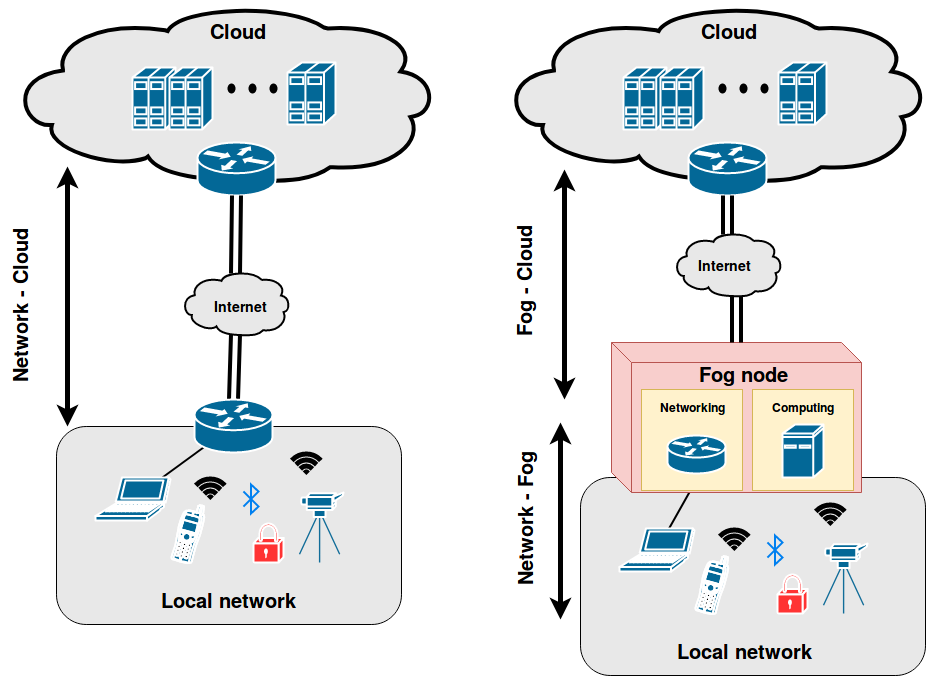
\includegraphics[scale=0.38]{pictures/fog}
\caption{Porovnání klasické a Fog architektury}
\label{obr.fog}
\end{center}
\end{figure}
 Zavedením principů Fog computingu vznikají pro síť následující výhody:
 \begin{itemize}
 \item \textbf{Zlepšení bezpečnosti} \cite{fog}
 
     Síťové prvky jsou trvale napájené a připojené k internetu. Podporují pokročilé
     bezpečnostní funkce, a proto je možné například vytvářet šifrované tunelové
     spojení pro bezpečný přenos dat.     
\item \textbf{Nižší nároky na šířku pásma a latenci} \cite{fog}

    Odeslaná data z koncových zařízení jsou zpracovávána a filtrována na okraji 
    sítě. Tím je možné rychleji reagovat na přijaté zprávy a snížit nároky
    na latency a šířku pásma. Zároveň krátkodobá data mohou být uložené ve 
    Fog vrstvě a centrální datové cetrum může být využito pro dlouhodobé údaje, 
    které se zpracovávají pokročilými algoritmy pro analýzu dat.
 \item \textbf{Jednotná správa} \cite{fog}
 
    Při správě sítě už se nemusí přistupovat přímo na koncové prvky, které 
    často komunikují různými protokoly, ale stačí pouze
    řídit síťová zařízení v jednotlivých Fog vrstvách, které odstiňují různorodost
    protokolů a nabízí standardizovaný přístup. Díky této abstrakci je 
    zároveň zjednodušeno zpracování získaných dat a je umožněno přímé zasílání zpráv
    mezi koncovými prvky, které používají odlišné komunikační protokoly.
 \end{itemize} 
 
 \subsection{IoT brána} 
 IoT brána je síťové zařízení, které je umístěno velmi blízko koncových zařízení
 a představuje vstup do Fog vrstvy. Jejím hlavním cílem je získávat data 
 z připojených zařízení a poskytovat je vyšším vrstvám. Pokud je brána reprezentována
 výkonnějším síťovým prvkem, tak v rámci brány může probíhat i základní zpracování
 dat. 
 
 Pro IoT sítě je typické, že obsahují velké množství koncových prvků komunikujících
 různorodými způsoby. Zejména senzory použivají protokoly, které nepodporují
 IP spojení. Důvodem použití této komunikace je často velký
 důraz na nízkou spotřebu a specifické požadavky na způsob zasílání zpráv.
 Příkladem protokolů pro senzorové sítě je například:
 Z-Wave, Bluetooth a Zigbee. Jejich detailní popis se nachází v kapitole \ref{protokoly}.
 Tato různorodost vyžaduje, aby brána obsahovala dodatečná rozhraní, které 
 umožní připojení nejrůznějších bezdrátových i drátových koncových prvků. 
 
 V součastné době existuje mnoho různých bran jejichž parametry se liší dle 
 způsobu nasazení a provozních nároků. Velkým problémem v této oblasti je malý 
 důraz na bezpečnostní funkce, které umožní vzdálené řízení brány, kontrolu provozu a 
 aktualizace programového vybavení. Z těchto důvodů vznikl opensource projekt BeeeOn \cite{beeeon}
 jehož cílem je vytvořit softwarou IoT bránu, kterou bude možné spustit na různých 
 hardwarových platformách. BeeeOn brána je navržena modulárně tak, aby byla schopna 
 zpracovávat více rozdílných senzorových protokolů, a tím bude možné provozovat jedno
 univerzální zařízení namísto několika proprietárních. Zároveň je kladen důraz na bezpečnost, 
 a proto veškeré údaje, které je možné získat o provozu, jsou poskytovány pro analýzu. Nad těmito údaji
 je postaven detekční algoritmus, který je výsledkem této diplomové práce.
 
 %přidat popis BeeeOn

 \subsection{Komunikační model a jeho hrozby}
 Při použití principů popsaných v předchzích kapitolách lze model komunikace rozdělit
 do následujících vrstev \cite{iotSurvey}:
 \begin{itemize}
 \item Aplikační vrstva 
 \item Síťová vrstva
 \item Senzorová vrstva
\end{itemize}
 Jednotlivé vrstvy budou popsány v následujích podkapitolách.
 
 \subsubsection{Senzorová vrstva}
 Senzorová vrstva obsahuje veškerá koncová zařízení, které získávají informace ze svého
 okolí nebo vykonávají potřebnou službu \cite{secFramework}. Tato zařízení jsou připojena
 kabelově nebo bezdrátově k IoT bráně. K jedné bráně může být připojeno několik
 prvků, které komunikují odlišnými způsoby.
 
 Velkým nebezpečím této vrstvy jsou zejména bezdrátové protokoly, protože při nepoužití
 zabezpečení může snadno dojít k odposlouchávání nebo úprávám provozu \cite{iotSurvey}.
 Dále se zde mohou vyskytovat zařízení, které jsou označeny jako zabezpečené, 
 ale používají zastaralé bezpečnostní funkce nebo obsahují implementační chyby. 
 Tento případ je velmi nebezpeční, protože vyvolává falešný pocit bezpečí.
 
 \subsubsection{Síťová vrstva}
 Po zpracování senzorových dat na bráně je nutné získané informace odeslat dalším
 službám. K tomuto účelu slouží síťová vrstva. Cílem této vrstvy je také umožnění 
 vzdálené správy brány \cite{secFramework}. Pro výběr konkrétního protokolu je 
 nutné znát rozhraní aplikační vrstvy. Nicméně spojení je většinou vytvořeno
 pomocí protokolu HTTPS (Hypertext Transfer Protocol Secure) nebo technologie
 VPN (Virtual Private Network). Nad tímto spojením je postaven další služba pro 
 výměnu zpráv. Příkladem může být: MQTT (Message Queuing Telemetry Transport),
 COAP (Constrained Application Protocol),
 AMQP (Advanced Message Queuing Protocol).
 
 Bezpečnostní hrozby této vrstvy jsou stejné jako v klasických sítích. Je potřeba
 dodržet principy důvěry, integrity a dostupnosti. Tímto přístupem je možné
 předejít útokům jako: DDoS (Distributed Denial Of Service),
 MITM (Man In The Middle) a podvržení informací. Zároveň je nutné
 nezapomenout, že se zde většinou vyskytuje M2M (Machine To Machine)
 komunikace a je důležité použít 
 vhodná komunikační rozhraní \cite{iotSurvey}.
 
 \subsubsection{Aplikační vrstva}
 Aplikační vrstva se stará o ukládání dlouhodobých dat a jejich finální zpracování. 
 Zároveň zobrazuje uživateli zpracované informace a umožňuje provádět konfiguraci
 celé sítě. Z důvodu možné rozsáhlosti celé sítě je kritické, aby správa
 topologie podporovala automatizaci. \cite{secFramework}.
 
 Tato vrstva je umístěna vetšinou v datovém centru a umožňuje vzdálený přístup. 
 Její bezpečnostní problémy lze přirovnat k problémům cloud computingu. Dle
 množství požadovaných funkcí může být různě složitá a s rostoucí složitostí
 se také liší nároky na úroveň zabezpečení. Příkladem možných útoků může být:
 Buffer Overflow, SQL Injection nebo DDoS.
 
 \newpage
 
 \section{Používané komunikační protokoly} \label{protokoly}
 Jedním z hlavích cílů IoT je možnost vzájemného propojení různých komunikačních protokolů, 
 které umožní automatizovanou výměnu zpráv mezi všemi dostupnými zařízeními. Tímto způsobem
 je následně možné zefektivňovat a usnaďnoat lidskou práci.
 
 V následujích podkapitolách bude popsána množina aktuálně často používaných protokolů
 včetně jejich bezpečnostních funkcí.
 
  \subsection{MQTT}
  MQTT je otevřený síťový komunikační protokol typu pulish/subcribe, který byl navržen
  v roce 1999. Již od návrhu byl zaměřen na nízkou náročnost komunikace a jednoduchost
  implementace. Díky těmto vlastnostem je velmi vhodný pro IoT a M2M systémy. \cite{mqtt}
  \subsubsection{Způsob komunikace}
  
  Protokol MQTT je postaven nad transportní vrstvou TCP (Transmission Control Protocol)
  a využívá model pulish/subcribe, který vychází z tradičního způsobu zasílání zpráv
  typu klient-server. Roli serveru zde plní speciální uzel, který se nazývá broker.
  Broker je známý všem ostatním klientům, kteří mohou zasílat zprávy pomocí operace
  \textit{publish} nebo se přihlásit o příjem zpráv díky operaci \textit{subscribe}.
  Na základě provedených operací broker přijímá zprávy a rozhoduje o jejich přeposlání.
  Způsob odeslání zprávy závisí na obsažených metadatech.
  
  Nejčastěji o směru odeslání rozhoduje předmět (topic) zprávy. Předmět je tvořen
  jednoduchým UTF-8 řetězcem s hierarchickou strukturou, ve které jsou jednolivé
  vrstvy odděleny dopředným lomítkem a každá z nich musí obsahovat minimálně jeden
  znak (např. domov/přízemí/světloŠatna). V předmětu
  zprávy mohou být některé vrstvy nahrazeny zástupnými symboly + a \#. Symbol + dokáže
  nahradit pouze jednu úroveň předmětu libovolným řetězcem a symbol \# umožňuje
  zastoupit více úrovní. Díky těmto symbolům mohou klienti odeslat nebo přijímat
  zprávy z více témat. Schéma topologie a ukázka využití předmětů zpráv se nachází na 
  obrázku \ref{obr.mqtt-arch}.
  
  \begin{figure}[ht]
\begin{center}
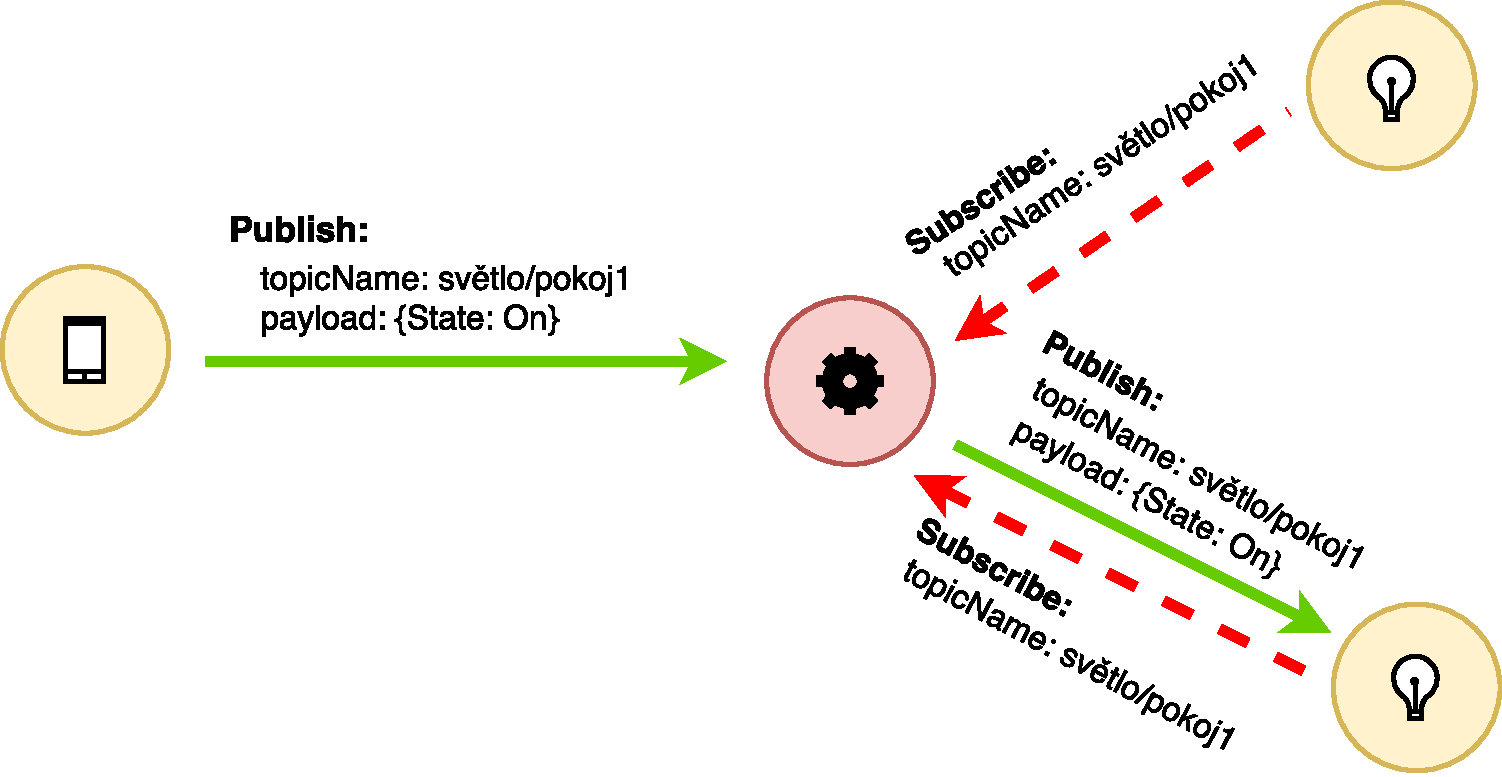
\includegraphics[scale=0.41]{pictures/mqtt-arch}
\caption{MQTT architektura}
\label{obr.mqtt-arch}
\end{center}
\end{figure}
  
  Další užitečnou položkou protokolu MQTT je QoS (Quality of Service),
  která může nabývat hodnot 0, 1 nebo 2.
  
   \begin{itemize}
    \item \textbf{QoS 0}
    
    Veškeré zprávy jsou odesílány bez potvrzení a žádným způsobem
    není zvýšena úroveň spolehlivosti, která je shodná se spolehlivostí protokolu TCP.
    
    \item \textbf{QoS 1}
    
    Pomocí potvrzování zajišťuje, že každá zpráva bude příjemci doručena alespoň jednou.
    
    \item \textbf{QoS 2}
    
     Umožňuje, aby každá zpráva byla spolehlivě doručena právě jednou.
   \end{itemize}
  Hodnota QoS se nastavuje vždy mezi dvěma uzly při navazování spojení.
  Z pohledu brokeru se může stát, že přijatá a odeslaná zpráva mají jiné QoS.
  Úrovně 1 a 2 dále umožňují perzistetní ukládání zpráv v případě, že příjemce je
  nedostupný. Zároveň platí, že s vyšší úrovní roste i režie komunikace. \cite{mqtt_intro}
 \subsubsection{Bezpečnost}
 Zabezpečení protokolu MQTT je možné rozdělit do následujících vrstev:
 \begin{itemize}
  \item \textbf{Síťová vrstva}
  
    Veškerá komunikace je postavena nad TCP/IP, a proto lze probíhající komunikaci
    zapouzdřit pomocí VPN připojení
    jako v běžných počítačových sítích. Kvůli větším nárokům na výkon je toto
    řešení vhodnější pro výkonější zařízení jako jsou například IoT brány, které
    mohou s brokerem navázat site-to-site spojení. \cite{mqtt_sec}
    
  \item \textbf{Transportní vrstva}
  
  Na této úrovni se využívá šifrování provozu pomocí protokolu TLS (Transport
  Layer Security). Omezením této metody jsou požadavky na výkon, které mohou být
  poměrně vysoké pokud nastává časté navazování spojení. \cite{mqtt_sec}
  
  \item \textbf{Aplikační vrstva}
  
  Samotný protokol MQTT nedefinuje žádné šifrovací mechanismy na aplikační úrovni. 
  Zabezpeční dat zde musí zajistit uživatel ještě před jejich zapouzdřením do MQTT zprávy. 
  Ovšem tímto způsobem je možné šifrovat jen tělo zprávy a hlavička zůstává nezměněná.
  
  Pro autentizaci je možné využít ověření pomocí jména a hesla nebo x.509 certifikátu.
  Jméno a heslo je přenášeno nešifrovaně, a proto je vhodné tuto metodu doplnit se 
  zabezpečením síťové nebo transportní vrstvy. Autentizaci pomocí certifikátů 
  je možné využít jen v případě použití TLS. Tato metoda je vhodnější pokud všechna
  zařízení jsou po jednotnou správou a je možné automatizovat distribuci 
  klientských certifikátů.
  
  Dále je na straně brokeru možné definovat pravidla pro autorizaci. Tyto pravidla 
  přiřazují klientů oprávnění pro provedení operací publish a subscribe
  nad příslušnými tématy. \cite{mqtt_sec}
  
 \end{itemize}

  \subsection{COAP}
  CoAP (Constrained Application Protocol) je otevřený přenosový protokol určený pro
  komunikaci síťových zařízení s velmi omezeným výkonem. Návrh vychází z RESTful
  (Representational State Transfer) principů, tudíž jeho použití je velmi vhodné
  v prostředích s již existujícím webových rozhraním, do kterého se snadno integruje. \cite{coap}
  
   \subsubsection{Způsob komunikace}
   Komunikace je postavena nad protokolem UDP (User Datagram Protocol) a vychází
   z modelu request/response, který se využívá u protokolu HTTP (Hypertext
   Transfer Protocol). Oproti protokolu HTTP je zde omezen počet možných operací
   a komunikace probíhá asynchronně. Dle důležitosti odesílané zprávy je možné určit,
   zda se má zasílat potvrzení či nikoli. Protože veškerá komunikace probíhá nad
   protokolem UDP, tak přenášené zprávy obsahují položku Message ID, která dokáže
   ošetřit duplikaci přijatých dat.
   %pokud to bude krátků můžu přidat option políčka pro udělání akce po splnění podmíky
   
   Pro zajištění integrace s běžnými webovými službami a zachování nízkých nároků
   se v CoAP topologii velmi často vyskytují proxy servery. Tyto servery mohou plnit
   funkci běžných reverzních a dopředných proxy, mapování mezi CoAP a HTTP protokolem
   nebo vyvažování zátěže. Způsob komunikace a schéma možné způsoby propojeí jsou na
   obrázku \ref{obr.coap-arch}. Senzor reprezentuje koncový prvek s omezeným výkonem.
   
   \begin{figure}[ht]
   \begin{center}
   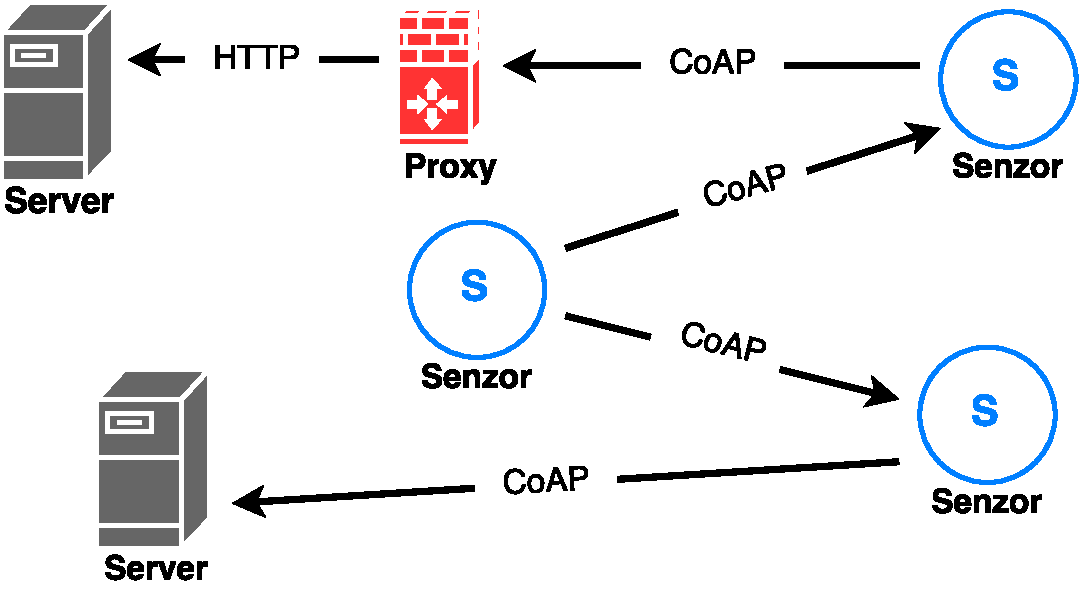
\includegraphics[scale=0.41]{pictures/coap-arch}
   \caption{CoAP architektura}
   \label{obr.coap-arch}
   \end{center}
   \end{figure}
   
   Ve specfikaci protokolu CoAP jsou definovány následující operace:
   \begin{itemize}
    \item \textbf{GET}
    
    Metoda \textit{GET} vrací aktuální stav požadovaného zdroje, který je identifikován pomocí
    URI (Uniform resource identifier). Tato operace je vždy bezpečná a idempotentní.
    
    \item \textbf{POST}
    
    \textit{POST} požadavek obsahuje ve svém těle novou reprezentaci cílového zdroje a požaduje 
    jeho zpracování. Funkce, která
    novou reprezentaci přijímá je definovaná na cílovém uzlu s příslušným URI.
    Výsledkem je vytvoření nového zdroje nebo aktualizace původního. Tato metoda
    není z pohledu zpracování bezpečná ani idempotentní.
    
    \item \textbf{PUT}
    
    Tato metoda specifikuje nový stav cílového zdroje, který specifikován použitým URI. Zdroj
    se buď vytvoří, nebo 
    v případě jeho existence aktualizuje. Provedení operace není bezpečné, ale 
    je idempotentní.
    
    \item \textbf{DELETE}
    
    Operace \textit{DELETE} požaduje smazání zdroje s příslušným URI. Tato metoda není bezpečná,
    ale je idempotentní.
    
   \end{itemize}
   
   Vyhledání potřebného zdroje je v topologii protokolu CoAP možné provést pomocí
   znalosti jeho URI nebo odesláním multicastového požadavku na definovanou
   skupinu uzlů. Možnost vyhledávání cílových zdrojů je velmi důležitá zejména
   v M2M prostředích. \cite{coap}
   
   \subsubsection{Bezpečnost}
   Samotný protokol nijak nedefinuje možnost autentizace a autorizace. V případě
   potřeby je nutné tyto mechanismy implementovat v aplikačním kódu. 
   
   Pro zajištění šifrování provozu nabízí CoAP následující režimy:
   \begin{itemize}
    \item \textbf{NoSec}
    
    Tento mód neobsahuje žádnou úroveň zabezpeční a veškeré zprávy jsou zasílány
    v otevřené podobě. 
    
    \item \textbf{PreSharedKey}
    
    V tomto případě se náváže spojení pomocí protokolu DTLS (Datagram Transport
    Layer Security), které využívá symetrické šifrování. Předsdílený klíč musí
    být známý všem uzlům před zahájením komunikace. 
    
    \item \textbf{RawPublicKey}
    
    Tento režim také navuzuje zabezpečené spojení pomocí protokolu DTLS, ale místo
    symetrické šifry se používá asymetrická.
    
    \item \textbf{Certificate}
    
    Mód \textit{Certificate} rozšiřuje \textit{RawPublicKey} o přidání certifikátu.
   \end{itemize}

   Podobně jako u protokolu MQTT je i zde možné ochránit provoz na síťové
   vrstvě pomocí VPN. Při nasazení libovolného režimu zabezpeční je nutné počítat 
   s většími nároky na výkon, které musí klient splňovat pro navazování a udržování 
   spojení. \cite{coap}
   
  \subsection{Z-Wave}
  
  Z-Wave je bezdrátový komunikační protokol určený pro senzorové sítě, který vysílá 
  v subgigahercových pásmech ISM (Industrial, Scientific and Medical). Veškeré komunikační
  prvky jsou certifikovány aliancí Z-Wave, která zároveň poskytuje technickou dokumentaci a
  licence pro vývoj. V současné době existují certifikace Z-Wave a Z-Wave Plus. 
  Z-Wave Plus zařízení obsahují nový chipset, který vylepšuje komunikační parametry
  sítě a zároveň je zpětně kompatibilní se staršími modely. \cite{z-plus}
  Otevřená implementace celého protokolu se nazývá OpenZWave \cite{openzwave}, která
  je vyvíjena komunitou. \cite{cesnet-survey} 
 
 \subsubsection{Způsob komunikace}
 V Z-Wave síti se může maximálně vyskytovat 232 uzlů, mezi kterými se vždy nachází jeden označený
 jako kontroler. Pro přidání libovolného zařízení do sítě musí být nejprve provedo příme spárování
 s kontrolerem. Během párovacího procesu nový prvek získá vlastní 8 bitový identifikátor (\textit{Node ID}) a 
 unikátní 32 bitový identifikátor sítě (\textit{Home ID}), který má již od výroby kontroler uložen v nepřepisovatelné paměti.
 Následné zasílání zpráv už nemusí probíhat přímo mezi senzorem a kontrolerem, ale zprávy mohou
 být přeposílány sousedními prvky, které jsou trvale napájené, čímž se velmi zvyšuje možná rozloha sítě. 
 Pro odebrání libolného zařízení je opět nutné zajisiti přimé spojení s kontrolerem a spustit odstraňovací
 proces. \cite{cesnet-survey}
 
 V rámci specifikace Z-Wave \cite{zwave-spec} je definován mechanismus pro určení dostupných příkazů. Každý senzor obsahuje
 svou definici tříd funkcionalit (\textit{Command Class}), které obsahují dostupné příkazy a formát odpovědi. Tyto definice
 jsou předány kontroleru během procesu párování. Příkladem může být třída \textit{Binary Switch}, která obsahuje příkazy:
 \begin{itemize}
 \item \textit{SET} - odesílá kontroler pro nastavení hodnoty 
 \item \textit{GET} - odesílá kontroler pro získání hodnoty  
 \item \textit{REPORT} - odesílá senzor jako odpověď na dotaz \textit{GET} 
 \end{itemize} 
 
 Při posílání zpráv je vždy vyžadováno potvrzení. V případě neobdržení potvrzení se vysílání opakuje. 
 Po třetím neúspěšném pokusu je požadavek zahozen.
 
 \subsubsection{Bezpečnost}
 Původní verze protokolu Z-Wave umožňovala volitelně využívat šifrování pomocí 128 bitového AES (Advanced Encryption Standard).
 Výměna symetrického klíče probíhá během počátečního párování, kde je vygenerovaný klíč šifrován pomocí výchozího
 klíče, který je uložen ve firmwaru. Vzhledem k tomuto postupu je dobré provádět počáteční párování na bezpečném
 místě, kde nemůže dojít k odposlechu. \cite{zwave-S0-attack}
 
 V roce 2016 Z-Wave aliance vydala nový S2 (Security 2) framework, který vylepšuje bezpečnostní funkcionality 
 a od roku 2017 je jeho použití povinné pro všechny nově certifikovaná zarízení. 
 
 S2 framework umožňuje zařízení rozdělit do následujících skupin s rozdílnými šifrovacími klíči:
 \begin{itemize}
  \item \textbf{Access Control} - 
   nejdůvěryhodnější třída, která obsahuje bezpečnostní prvky jako jsou například zámky,
   které zároveň podporují autentizaci
  \item \textbf{Authenticated} - 
  skupina určená pro běžné senzory, které podporují autentizaci 
  \item \textbf{Unauthenticated} - 
  třída pro ostatní prvky, které nepodporují autentizaci.
 \end{itemize}
 Autentizace probíhá pomocí PIN (Personal Identification Number) nebo QR (Quick Response) kódu.
 Výměna klíče je založena na algortmu ECDH (Elliptic-curve Diffie–Hellman), který zajišťuje 
 dostatečnou úroveň bezpečnosti během párovacího procesu. \cite{cesnet-survey}

 
  \subsection{BLE (Bluetooth Low Energy)} %!!! chybi citace
  BLE je bezdrátový prtokol určený pro senzorové sítě s důrazem na nízkou spotřebu. Byl představen 
  v roce 2010 jako součást specifikace Bluetooth 4.0 a je nekompatibilní s původními verzemi. 
  Za vývoj a údržbu protokolu je odpovědná skupina Bluetooth SIG (Special Interest Group).
  V současné době je nejnovější verzí Bluetooth 5.
  
  \subsubsection{Způsob komunikace}
  BLE vysílá v bezlicenčním ISM pásmu na frekvencích od 2.4 GHz do 2.4835 GHz. Specifikace
  protokolu vychází z Bluetooth, ale zejména díky změnám parametrů v rádiové vrstvě 
  jsou navzájem nekompatibilní. Do verze 4 umožňuje navázat pro koncová zařízení pouze jedno spojení,
  a proto 
  vytváří hvězdicovou topologii s jedním centrálním prvkem. Od verze 5 je možné využívat více připojení
  a lze vytvořit flexibilnější mesh topologii. 
  
  Před zahájením komunikace mezi centrálním prvkem a senzory je nutné nejprve prvést párování, 
  které probíhá v následujících krocích:
  \begin{itemize}
   \item \textbf{Vysílání žádostí}
   
   Při spuštění párování začně koncový prvek na kanálech určených pro propagaci všesměrově vysílat žádosti o připojení,
   které obsahují název zařízení, jméno výrobce a podporované služby.
   
   \item \textbf{Přijímání žádostí}
   
   Pokud je centrální prvek přepnutý do párovacího režimu, tak naslouchá příchozím požadavkům, které zobrazuje uživateli.
   Po výběru správného zařízení se ukončí mód naslouchání a začne se navazovat spojení.
   
   \item \textbf{Inicializace připojení} 
   
   Během této fáze se obě strany domlouvají na parametrech komunikace.
   \item \textbf{Komunikace}
   
   Po úspěšném navázání spojení je možná na základě dostupných služeb provádět zasílání zpráv.
  \end{itemize}

 
   \subsubsection{Bezpečnost}
   BLE umožňuje volitelně používat šifrování pomocí AES, jehož šifrovací klíč je 
   vytvořen behěm párování v části inicializace připojení. Velmi důležité je zabezpečit 
   výměnu sdíleného klíče, která až do verze 4.1 není bezpečná, protože neumožňuje ochranu
   před odposloucháváním. Vylepšení přichází až od verze 4.2, ve které lze využít ECDH.
   
   Vzhledem k různorodosti možných typů zařízení definuje BLE následující kategorie
   určující způsob výměny klíče:
    \begin{itemize}
     \item \textbf{Just Works}
     
     Nejjednodušší třída, která provádí výměnu automaticky a zároveň má nejmenší nároky 
     na připojované zařízení, které nemusí podporovat autentizaci. Díky chybějící autentizaci 
     je tato metoda zranitelná vůči MITM (Man in the middle) útokům.
     \item \textbf{Out of Band}
     
     V této kategorii jsou veškeré klíče vyměňovány odlišným komunikačním kanálem např. přes NFC (Near Field Communication).
     Celková bezpečnost této metody závisí na důvěryhodnoti použitého kanálu.
     \item \textbf{Passkey}
     
     Tato metoda vylepšuje \textit{Just Works} o autentizaci, která spočívá v uživatelském zadání šesti 
     místného kódu. Pro ochranu před odposlouchávání musí být použit algoritmus ECDH, který je dostupný
     až od verze 4.2.
     
     \item \textbf{Numeric Comparison}
     
     Využití tohoto způsobu párování je možné pouze od verze 4.2. Dochází zde k rozšíření metody \textit{Just Works}
     o jeden kontrolní krok, který slouží jako ochrana před MITM útokem. Po výměně klíčů každé zařízení
     vygeneruje šestimístný číselný kód, který následně zobrazí uživateli a čeká na jeho potvrzení.   
     
    \end{itemize}

   
   \newpage
 % popis a bezpečnostní analýza ZWave a Bluetooth
  \section{Bezpečnostní slabiny}
  Na základě provedené analýzy aktuálně používaných protokolů budou v této kapitole 
  popsány jejich bezpečnotní slabiny, které budou později využity při návrhu 
  detekčních algoritmů. Jelikož je tato práce zaměřena na senzorové protokoly 
  nekumunikující přes IP, budou v této kapitole popsány slabiny protokolů 
  Z-Wave a BLE.
  
 \subsection{Z-Wave}
 Hlavním problém jsou zařízení certifikovaná před březnem 2017, jelikož nepodporují S2 framework.
 Tyto prvky nemusí při své komunikaci využívat žádnou formu šifrování a síť se tak stává 
 velmi zranitelnou. V minulosti již bylo provedeno několik útoků, které pomocí projektu
 Scapy-Radio projektu \cite{ezwave} nebo knihovny OpenZWave  byly schnopny ovládat jednotlivé senzory. 
 %\cite{openzwave-attack}
 Při využití šifrování je velmi zranitelná doba během párovacího procesu, jelikož je při výměně
 šifrovacích klíčů použit výchozí klíč uložený ve firmware zařizení. Zároveň se 
 u jednoho typu zámku podařilo objevit implementační chybu \cite{zwave-S0-attack}, které umožňovala vnutit 
 nový šifrovací klíč a převzít tak kontrolu nad senzorem. 
 
 Při využití S2 frameworku dosud nebyly objeveny žádné zranitelnosti, ovšem tento
 framework je poměrně nový a většina používaných zařízení byla certifikována 
 ještě před jeho zavedením.
 
 \subsection{BLE}
 Velkou hrozbou jsou zařízení s verzí 4.1 nebo nižší, protože nepodporují žádnou ochranu před 
 odposlouchávání a MITM útokům v době párování. Od verze 4.2 je již pro výměnu klíčů použit ECDH 
 algoritmus, který zabraňuje možnému odposlouchávání, ale v případě použítí párovací metody, které
 nepodporuje autentizaci není zajištěna ochrana před MITM útoky.  \cite{cesnet-survey}
 
 Dalším problémem jsou samotní výrobci, kteří často nevyužívají bezpečnostní funkce protokolu  \cite{ble-locks} nebo
 implementují vlastní způsoby zabezpečení na aplikační úrovni. Tímto dochází k nezabepečení fáze 
 párování a často se vyskytují i implementační chyby, které přinášení další zranitelnosti \cite{ble-attack} a
 umožňují útočníkovi získat kontrolu nad celým provozem.  \cite{cesnet-survey}
 
 Nevýhodou je velmi dlouhá a komplikovaná specifikace protokolu, která vede k implementačním 
 chybám samotného BLE \cite{blueborne}. Tím vzniká nebezpečí, že i u výrobce, který využívá
 všech bezpečnostní funcionalit,
 se mohou vyskytovat zranitelnosti díky chybné implementaci komunikačních vrstev protokolu. \cite{cesnet-survey}
 
 \newpage
 \section{Možnosti detekce}
 V běžných IP sítích se pro detekci hrozeb nejčastěji používají IDS (Intrusion Detection System) a
 IPS (Intrustion Prevention System) systémy. Tyto služby rozšiřují koncept klasického firewallu, který
 blokuje nebo povoluje síťový provoz na základě statických pravidel, o podrobnější sledování 
 datových toků, které jsou zablokovány na základě nestandartního chování.
 
 IDS/IPS může být reprezentováno samostatným hardwarovým zařízením nebo softwarovým programem, který
 může být dále rozšířen o monitorovací sondy, které se starají pouze o sběr dat a jejich odesílání
 pro následnou analýzu. Zároveň
 se může lišit i umístění v síti. Detekční systémy lze provozovat před hraničním směrovačem 
 a detekovat tak kompletní příchozí a odchozí data nebo za hraničním směrovačem, což 
 umožní vyhodnocovat jen vyfiltrovaný provoz. Případně je možné nasadit IDS/IPS přímo na koncové
 stanice, kde kromě síťových dat lze získávat i informace o běhu systému. Poslední způsob poskytuje
 nejvíce detailní možnost analýzy, protože se provádí na míste vzniku komunikace a případný útok
 je možné zastavit již při jeho vzniku a zabránit případnému rozšíření. Nevýhodou takového nasazení
 je ztráta celkového pohledu na síť. Při zavedení IDS/IPS systému je z těchto důvodů dobré 
 kombinovat způsoby nasazení a umožnit vzájemné sdílení detekovaných incidentů.
 
 %\section{Metody zpracování}
 Při zaměření na zpracovávání datových toků lze dekteční systémy rozdělit do dvou základních kategorií:
 \begin{itemize}
  \item \textbf{Detekce anomálií}
  
  Tato metoda je založena na statistickém modelování. Nejprve se vytvoří profil běžného chování sítě, 
  který se následně porovnává s aktuálním provozem. Dle použité metody se může profil běžného provozu
  průběžně aktualizovat. Pokud měřené hodnoty síťového provozu překročí hodnotu stanoveného profilu
  nad definovaný limit, tak je detekován incident. Výhodou metody anomálií je její uplatnění i na 
  dosud neznámé útoky. Tento princip zároveň způsobuje větší míru falešných poplachů, a proto 
  je nutné jejich pečlivější ověření. Příkladem detekčních metod je: strojové učení, časové řady nebo
  stavové automaty \cite{ids-ips}.
  
  \item \textbf{Detekce signatur}
  
  V případě použítí této metody je využíváno signatur (profilů) předem známých útoků. Výhodou je, že díky 
  popsaným signaturám je tato metoda poměrně přesná a detekuje málo falešných incidentů. Naopak
  nevýhodou je, že není možné detekovat nové druhy útoků, pro které není známý profil. Problémem
  také je, že signatury musí být uloženy na nějakém perzistetním úložišti, které je dostupné 
  lokálně nebo vzdáleně \cite{ids-ips}.
 \end{itemize}
 
 %\section{Možnosti detekce}
 IoT sítě k běžnému IP provozu přidávají senzorové protokoly, jejichž chování je také dobré monitorovat, 
 protože jsou připojeny do počítačové sítě a mohou být zneužity při útocích. Bohužel detekční metody 
 nejsou pro tyto sítě moc rozšířené, a tím dochází ke zvýšení rizika a dopadu možných útoků. Pro určení 
 incidentů lze využít stejných principů jako v IP sítích, ale liší se způsob získávání dat pro analýzu. 
 Pro sběr informací lze využít následující přístupy:
 \begin{itemize}
  \item \textbf{Testbed}
  
    Tato metoda spočívá ve vytvoření specializovaného prostředí, ve kterém se nachází pouze testované 
    a měřící zařízení. Cílem je ověřit, že nově připojovaný senzor splňuje veškeré bezpečnostní 
    požadavky a neobsahuje žádné známe zranitelnosti. Měřící prvky reprezentují nástroje, které 
    jsou schopné odposlouchávat komunikaci a využívájí se také například při automatizovaných
    penetračních testech.   
  \item \textbf{Externí sonda}
  
  Funkce sondy je stejná jako v IP sítích. Jedná se o samostatné zařízení umístěné v sítí, které
  umožňuje sledovat probíhající komunikaci a odesílat získatné údaje ke zpracování. 
  Výhodou je velké množství, které lze získat, ale zároveň komplikací je šifrovaný provoz
  a často i cena kvalitní sondy.
  Dalším využitím 
  může být honeypot, kdy se sonda tváří jako zranitelný prvek a reportuje veškeré pokusy o útok.
    
  \item \textbf{Provozní statistiky}
  
  Posledním způsobem je sběr dat z příslušných rozhraní na IoT bráně. Tento postup nevyžaduje použití
  žádného dalšího zařízení, ale potřebuje, aby brána umožňovala získávat tyto statistiky. 
  Statistiky nejsou tak podrobné jako u externí sondy, ale výhodou je, 
  že získávání aktuálních dat o provozu je poměrně nenáročné.
 \end{itemize}
 
 Každá z předchozích metod používá jiný styl sběru dat. Při reálném použití je dobré vyhodnotit 
 bezpečnostní rizika a hrozby, podle kterých lze jednotlivé metody vhodně kombinovat.

 \newpage
 \section{Existující řešení}
 V součastnosti veškerá dostupná řešení se zaměřují na detekci útoků v IP protokolech. Mezi 
 současnými IDS/IPS systémy existují signatury pouze pro SCADA (Supervisory Control And Data Acquisition)
 protokoly. Pakon
 
 
 
  \begin{itemize}
 \item Existuje řešení pomocí Suricata, které používá Turris (centrální, signature
 based řešení)
 \item Neexistuje řešení, které by provádělo detekce z senzorových dat
 \item Neexistuje řešení, které by umožňovalo senzorové nebo pokročilé síťové
 detekce na bráně nebo mimo ni
\end{itemize}
 % aktuální řešení funguje na cetrálním monitorovacím prvku, které monitoruje IP
 % teprve nedávno vznikly signatury pro SCADA
 \section{Analýza požadavků}
 
  \subsection{Funkční požadavky}
  \subsection{Nefunkční požadavky}
 
 \section{Zvolené řešení}
 povídání o nutnosti učení se, ... další poznámky z telefonu



\chapter{Návrh}
Kapitola se zabývá návrhem způsobu detekce anomálií v~IoT sítích, který s~pomocí NEMEA
systému rozšiřuje bránu BeeeOn. Nejprve je popsána celková architektura a
možné způsoby nasazení. Dále následuje popis jednotlivých komponent detekčního systému.
V~závěru jsou identifikovány možné scénáře útoků.

  \section{Architektura}
 Cílem této práce je vytvoření programu, který bude schopen detekovat anomální provoz v IoT sítích. 
 Vzhledem k hardwarovým omezením, které můžou na IoT branách nastat, je architektura navržena tak, aby
 měla co nejmenší nároky na dostupné prostředky. Schéma nasazení detekčního systému se nachází
 na obrázku \ref{obr.deploy-arch}
 
 \begin{figure}[ht]
   \begin{center}
   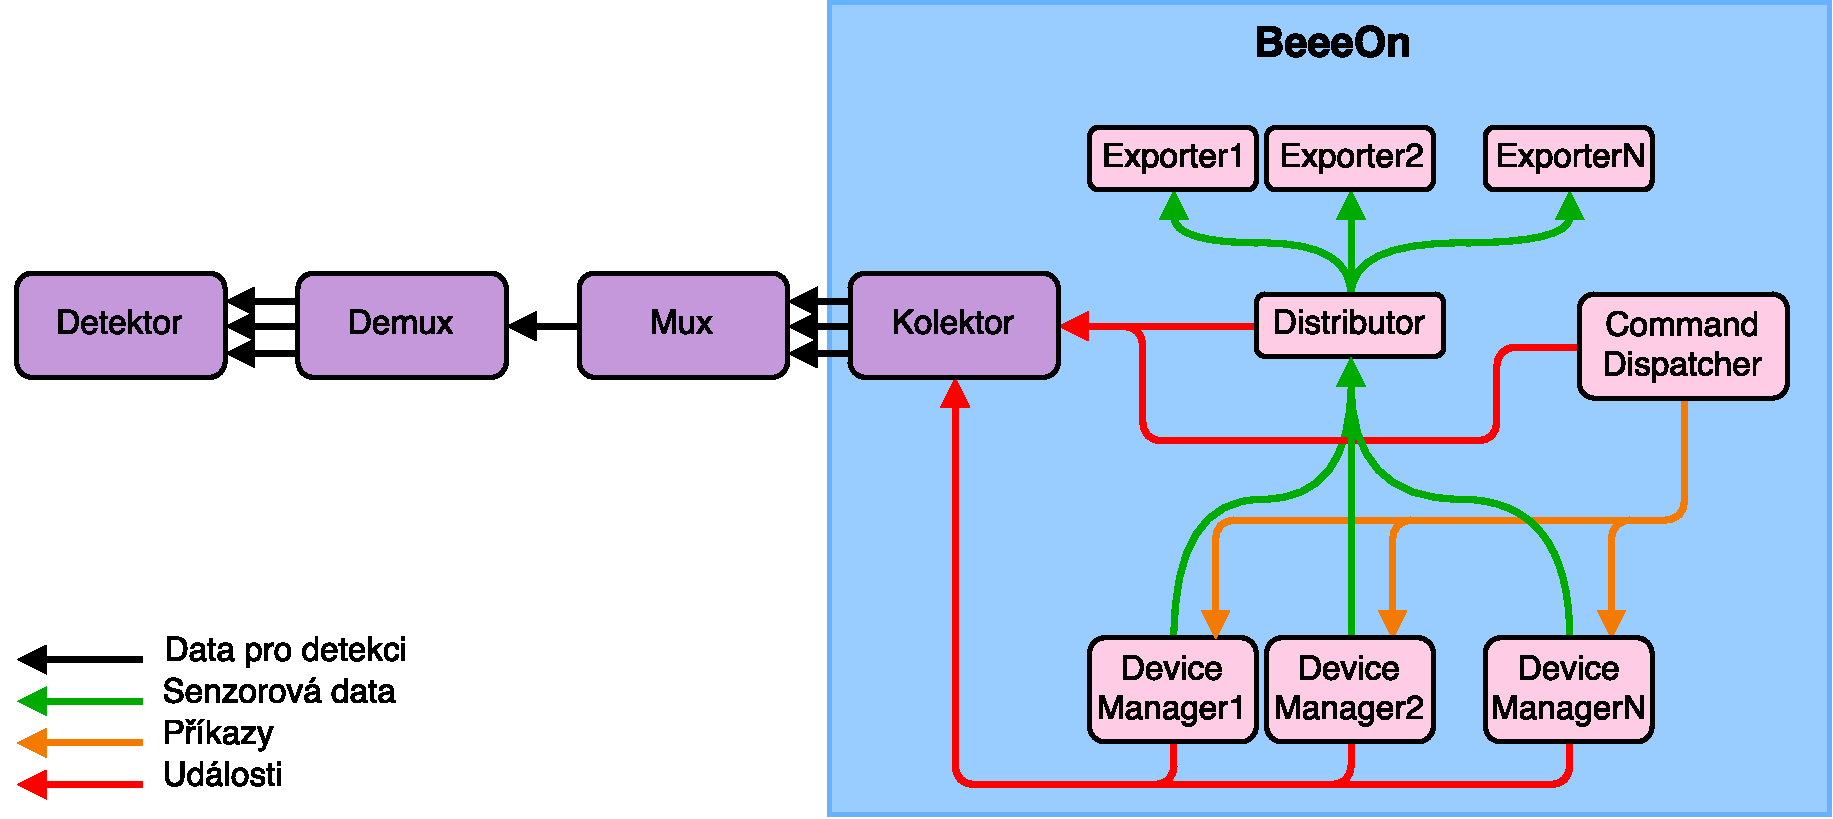
\includegraphics[scale=0.41]{pictures/deploy-arch}
   \caption{Architektura detekčního systému}
   \label{obr.deploy-arch}
   \end{center}
   \end{figure}
 
 Implementace BeeeOn brány obsahuje pro zpracování senzorových dat následující komponenty:
 \begin{itemize}
  \item \textbf{DeviceManager}:
    komponenta definovaná pro každý senzorový protokol, která implementuje veškerou komunikaci
    a zpracování dat
    
  \item \textbf{Distributor}:  
  přijímá data od \textit{DeviceManageru}, která nasledně předává příslušnému \textit{Exporteru}
  
  \item \textbf{Exporter}:
  implementuje protokol, kterým jsou data odesílány z brány
  
  \item \textbf{CommandDispatcher}:  
  komponenta, která přijímá uživatelské příkazy a distribuuje je cílovým komponentám
  
 \end{itemize}
 
 Každá z komponent v BeeeOn bráně navíc využívá návrhový vzor Observer, pomocí kterého jsou
 definovany události poskytující informace o každé komponentě. 
 Tímto způsobem bude vytvořený kolektor zíkávat data o provozu, která
 převede do fomátu UniRec (Unified Record) a pomocí systému NEMEA je odešle k analýze.
 
 Exportované informace o provozu bude přijímat detektor, který následně provede jejich zpracování a 
 vyhodnocení stavu. Všechny vytvořené komponety vytvořené pro detekci budou používat rozhraní 
 NEMEA. Díky tomu bude možné komponenty flexibilně provozovat na jednom nebo více různých zařízeních.
 Oddělené nasazení je důležité zejména pro brány s omezenými prostředky, které mohou provádět 
 pouze export dat a o vyhodnocení se bude starat odlišné zařízení s dostatečným výkonem. V případě 
 provozování více bran lze brány používat jako exportéry a veškerá získaná data zpracovávat 
 centrálně. 
 
 Kolektor pro každou událost vytvoří samostnatné výstupní rozhraní. Protože událostí může být 
 velké množství, tak bude vytvořen modul \textit{Mux}, který všechny výstupní rozhraní spojí do jednoho. 
 Pro zpětné rozdělení na jednotlivá rozhraní budou dloužit modul \textit{Demux}. Tyto moduly budou velmi užitečné
 zejména v případě kdy kolektor a detektor budou na rozdílných síťových prvcích, protože údaje 
 o provozu budou přenášeny přes počítačovou síť a bude vyžadováno zabezpeční všech odchozích
 rozhraní. S využítím \textit{Mux} a \textit{Demux} modulů bude stačit zabezpečit pouze jedno sjednocené rozhraní. 
 
 Výhodou návrhu řešení je flexibilita a modularita. Každá komponenta vždy samostatně pokrývá pouze jednu
 část detekčního systému a se díky NEMEA se každá z nich může nacházet na různých síťových prvcích. Zároveň
 v případě potřeby lze vytvořit další moduly, které budou rozšiřovat stávající funcionalitu.
 Podrobnější popis návrhu nově vytvořených komponent detekčního systému se nachází v následujících kapitolách.
 
 \section{Kolektor}
 Úkolem kolektoru bude sběr dostupných dat a jejich odeslání k následné analýze. Informace o 
 provozu budou sbírány z jednotlivých komponent BeeeOn brány, které jsou zpřístupňovány pomocí 
 návrhového vzoru Observer. Z tohoto důvodu bude kolektor vždy přímou součástí BeeOn brány. 
 Návrh struktury kolektoru je na obrázku 
 
 \begin{figure}[ht]
   \begin{center}
   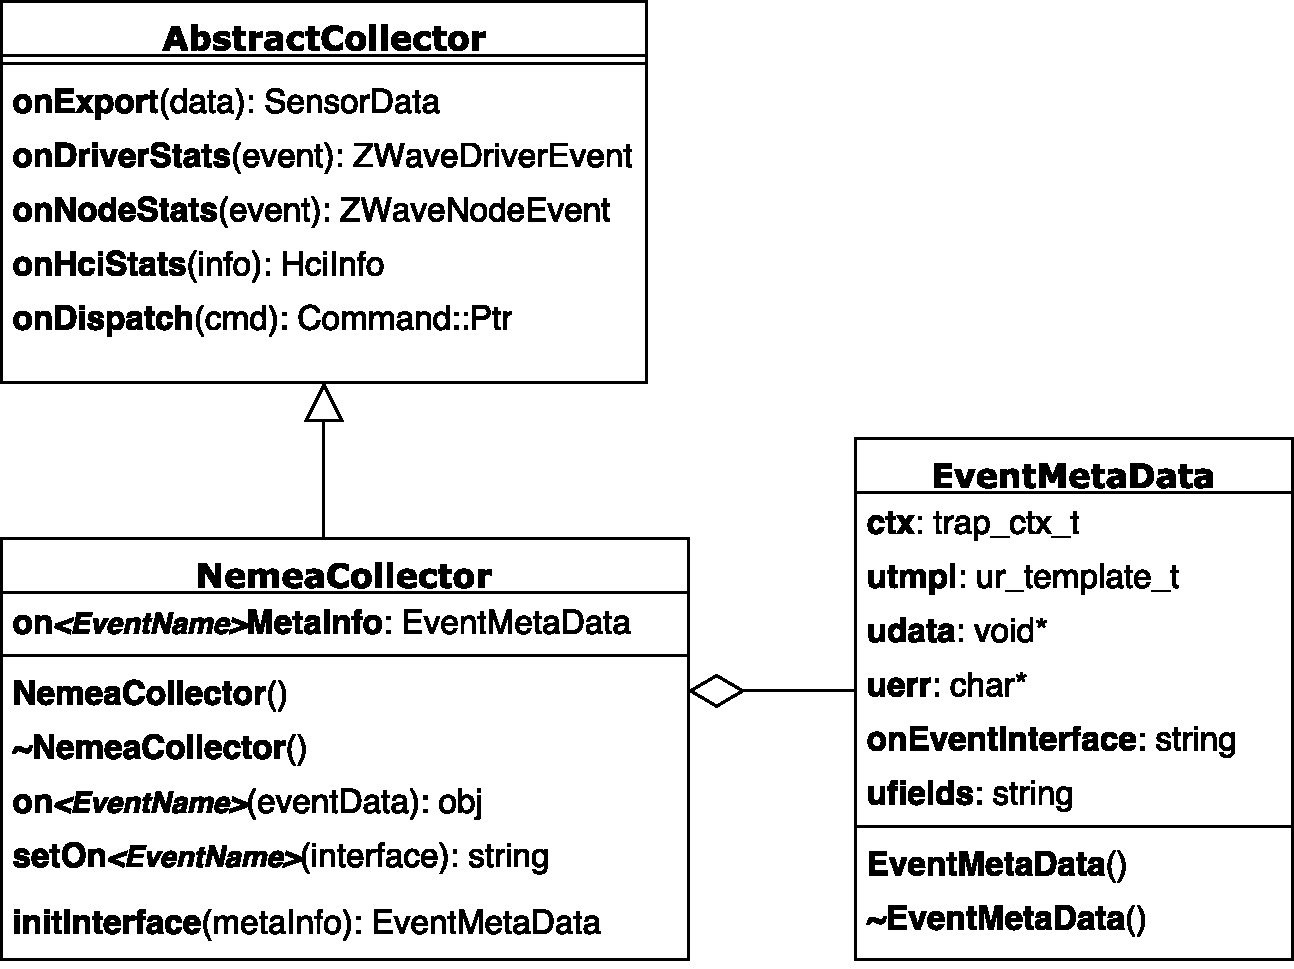
\includegraphics[scale=0.5]{pictures/modelTrid}
   \caption{Návrh kolektoru provozních dat}
   \label{obr.modelTrid}
   \end{center}
   \end{figure}
 
 obecné povídání o kolektoru - je vždy součástí brány
 návrh method a tříd v bráně
    
 \section{Detektor}
  časové řady
  univerzální návrh který umožňuje použití více nebo jen jednoho detektoru
  Sytaxe konfiguračního souboru - klíč hodnoty
  návrh metod a tříd 
  
 \section{Multiplexor a demultiplexor}
 
 \section{Scénáře útoků}


\chapter{Realizace}
Obsahem kapitoly je popis realizace nejzajímavějších částí vytvořeného programu. Pro zajištění
efektivity a snadné přenositelnosti byla veškeré implementace provedena v~jazyce C++, ve kterém
je zároveň napsána BeeeOn brána. Detekční systém přináší pouze jednu novou závislost a tou je NEMEA framework.
Ostatní použité knihovny se shodují s~již použitými v~BeeeOn bráně.

 
\section{Integrace kolektoru}    
     Vytvořený kolektor provozních dat je přímou součástí již existujícího projektu BeeeOn, a~proto jej bylo nutné 
     integrovat do spouštěcího procesu brány. Pro zajištění společné kompilace byly do souborů 
     \textit{CMakeLists.txt} přidány cesty ke zdrojovým souborům kolektoru a závislosti na knihovny
     z~NEMEA frameworku. K~určení způsobu spouštění jednotlivých komponent používá BeeeOn
     soubor \textit{factory.xml}. V~tomto souboru byla vytvořena nová komponenta s~názvem 
     \textit{collector}, 
     která byla následně přidána pod označením \textit{listener} do specifikace ostatních komponent.
     Toto nastavení 
     umožňuje přijímání definovaných událostí v~rámci návrhového vzoru \textit{Observer}.
     Samotná komponenta \textit{collector}
     obsahuje ve svém popisu seznam jmen událostí, kterým přiřazuje pojmenování výstupního \textit{libtrap}
     rozhraní. Formát názvu výstupu je vždy ve tvaru \textit{event-<názevUdálosti>}. 
     
     Vytvořené názvy událostí jsou při spouštění programu pomocí C++ reflexe předány třídě kolektoru
     \textit{NemeaCollector}. Tato třída používá již vytvořené makro \textit{BEEEON\_OBJECT\_TEXT},
     které pro definované 
     typy událostí volá přiřazené členské funkce. Každá událost má členskou funkci s~názvem ve formátu 
     \textit{set<názevUdálosti>()} přijímající jeden vstupní parametr typu string s~názvem výstupního 
     komunikačního rozhraní. V~rámci volání se do instance třídy \textit{EventMetaData}
     nastaví specifické hodnoty členských
     atributů o~daném typu události. Následuje volání členské funkce \textit{initInterface()},
     která přijímá vytvořenou instanci třídy  \textit{EventMetaData} a
     jednotně inicializuje všechny potřebné struktury pro odesílání dat.
     
     Po úspěšném nastavení všech částí se už jen v~rámci návrhového vzoru \textit{Observer} volají
     členské funkce událostí, které jsou definované ve třídě \textit{AbstractCollector} a implementované
     ve třídě \textit{NemeaCollector}. Získané informace z~brány jsou vkládány do UniRec zprávy a odeslány
     výstupním rozhraním.
     
\section{Mux a Demux}    

 Modul \textit{Mux} očekává na vstupu přepínač \textit{-i}, který ve formě řetězce určuje dostupná 
 komunikační rozhraní 
 zajištěná knihovnou \textit{libtrap}. Poslední identifikátor v~zadaném řetězci označuje jméno 
 výstupu. Druhým parametrem je \textit{-n}, který odpovídá počtu vstupních komunikačních
 rozhraní. Při spuštění 
 se pro každý vstup vytvoří samostatné vlákno pomocí knihovny OpenMP. Jelikož je veškerý provoz 
 odesílaný jedním společným výstupem, bylo nutné funkci \textit{trap\_ctx\_send()} vložit do
 kritické sekce, 
 protože pracuje se sdílenými strukturami pro všechny vlákna.
 
 Společná spojení mezi vytvořenými moduly \textit{Mux} a \textit{Demux} používá nastavený typ
 \textit{TRAP\_FMT\_RAW},
 který umožňuje posílat zprávy ve vlastně definovaném formátu. Hlavička vytvořeného formátu
 obsahuje: identifikátor druhu zprávy, číslo komunikačního rozhraní a typ formátu. Obsah přijatých zpráv
 je zapouzdřen do záhlaví. \textit{Mux} při každém přijetí dat kontroluje návratový
 kód funkce \textit{trap\_ctx\_recv()}, který identifikuje nový formát přijatých zpráv. Pokud
 dojde k~detekování změny, tak se pošle \textit{hello} zpráva s~upraveným popisem rozhraní.
 V~ostatních případech se jen přeposílají zapouzdřená data.
 
 Modul \textit{Demux} vyžaduje stejné přepínače jako \textit{Mux}. Jediným rozdílem je, že 
 název společného komunikačního rozhraní, které má \textit{Mux} na posledním místě, musí být zde uveden 
 jako první. Důvodem je, že knihovna \textit{libtrap} zpracovává nejprve vstupní a pak
 výstupní rozhraní. 
 
\section{Zpracování zadaných parametrů}

Načtení konfiguračního souboru má na starosti třída \textit{ConfigParser}, která pomocí parametrického
konstruktoru přijímá název konfiguračního souboru. Následně je možné volat členskou funkci
\textit{parseFile()}, která zpracovává jednotlivé konfigurační řádky a plní připravené struktury.
Zároveň jsou inicializovány pole pro uchovávání vypočtených profilů.
Jejich délka je specifikována preprocesorovou direktivou \textit{\#define DYNAMIC}.
 
Pokud byly zadány parametry pro pravidelný export dat, tak se při inicializaci potřebných struktur
zavolá funkce s~názvem \textit{initExportInterfaces()}, která vytvoří příslušná výstupní komunikační 
rozhraní. Jejich název je vždy vygenerován v~následujícím formátu: 
\textit{u:export-<názevKlíče><idKlíče>}. V~opačném případě se tato inicializace přeskočí a žádné
výstupní komunikační rozhraní pro export dat není vytvořeno.
   
\section{Výpočet profilu} \label{profileDef}
Veškeré přijaté údaje z~kolektoru jsou v~rámci detektoru ukládány do časových řad. Nad těmito 
daty jsou prováděny výpočty profilů, které využívají detekční funkce. Jelikož jsou profily
přepočítávány s~každým nový prvkem v~časové řadě, tak je důležité provádět výpočty efektivně, 
aby nemusela být vždy procházena celá řada při změně jedné hodnoty. Během implementace byly
vytvořeny členské funkce pro výpočet následujících částí profilu: průměr, klouzavý průměr, klouzavý rozptyl a
klouzavý medián. Tyto členské funkce jsou popsány v~níže uvedených sekcích.

\begin{itemize}
 \item \textbf{getMovingMedian()}%(\textit{sensor\_it, meta\_it, ur\_field, ur\_id})}
 
 
 Klouzavý medián značí hodnotu běžného mediánu odpovídající prvkům umístěných v~časové řadě. 
 Pro jeho výpočet je nutné udržovat položky aktuálního časového okna v~seřazeném pořadí.
 Při vkládání nového prvku je potřeba najít nejstarší prvek v~poli a nahradit ho nově přijatým. 
 Po provedeném nahrazení se pole může nacházet v~neseřazeném stavu a~je 
 vyžadováno jeho opětovné seřazení.
  Tato operace není náročná, protože se změní vždy jen jeden prvek, který je nutné
 přesunou na správné místo. Celková složitost začlenění nového prvku je $O(n)$, protože operace 
 nalezení a seřazení lze provést v~lineárním čase. Paměťové nároky vyžadují alokování dodatečného
 místa, které obsahuje kopii časové řady.
 
 Dále je potřeba zjistit, zda je časová řada sudé nebo liché délky. Pokud je lichá, tak se jako 
 medián vrátí její prvek umístění ve středu. V~opačném případě je výsledkem průměr dvou prostředních
 hodnot.
 
 Aby mohly být provedeny veškeré popsané operace, tak členská funkce pro výpočet mediánu
 potřebuje tyto vstupní parametry:
 \begin{itemize}
   \item \textbf{sensor\_it} -- iterátor na časovou řadu daného UniRec pole
   \item \textbf{meta\_it} -- iterátor na meta informace o~daném UniRec poli
   \item \textbf{ur\_field} -- řetězec s~názvem zpracovávaného UniRec pole
   \item \textbf{ur\_id} -- číselný identifikátor přijatého UniRec pole
 \end{itemize}
 
 \item \textbf{getMovingAverageAndVariance()}%(\textit{ur\_field, ur\_id, meta\_it, sensor\_it, meta\_id})}
 
 Tato členská funkce je zaměřená zejména na získání klouzavého rozptylu, ale v~rámci jeho výpočtu je možné
 získat i hodnotu klouzavého průměru, a proto jsou v~návratové hodnotě vráceny oba výsledky.
 Stejně jako v~předchozí sekci klouzavý rozptyl i průměr jsou odvozeny z~aktuálního časového
 okna celé řady.
 Průběh
 zpracování údajů probíhá s~ohledem na vstupní data, která 
 jsou reprezentována stále se posouvajícím časovým oknem. 
 
 Pro umožnění efektivního výpočtu se používá několik pomocných paměťových struktur. První z~nich 
 jsou dvě pole \textit{x} a \textit{x2} se shodnou velikostí jako má hlavní časová řada. Do pole
 \textit{x} jsou ukládána
 nově příchozí data a \textit{x2} udržuje jejich druhé mocniny. Dále je nutné ukládat součty
 hodnot v~těchto polích, které jsou uchovávány v~proměnných \textit{SX} a \textit{SX2}.
 
 V~rámci učící fáze detektoru jsou i zde příchozí prvky postupně vkládány do připravených struktur.
 Pokud jsou již pomocná pole naplněná, tak se při příchodu nové položky používá funkce
 \textit{rotate()}, která provede levou rotaci prvků a umístí nejstarší prvek na konec. Tento
 prvek je poté nahrazen nejnovější hodnotou. Součty jednotlivých polí jsou upraveny podle 
 následujícího předpisu:  
 \[
  součetPole + novýPrvek - nejstaršíPrvek
\]
 
 Po upravení pomocných struktur je možné provést finální výpočet. Průměr je snadno získán vydělením
 udržovaného součtu počtem prvků v~časovém okně (\textit{N}). Pro určení hodnoty rozptylu se provádí
 následující operace:
\[
   \frac{N * SX2 - SX * SX}{N * (N - 1)}
\]
Pro získání veškerých údajů pro popsané výpočty přijímá členská funkce stejné vstupní parametry
jako \textit{getMedian()} a navíc je ještě očekávána hodnota \textit{meta\_id}, která určuje, 
zda bude v~rámci metadat použita skupina \textit{metaData} nebo \textit{metaProfile}.
Tyto skupiny byly diskutovány v~dřívější Sekci \ref{configParam}.


 \item \textbf{getOverallAverage()}%(\textit{sensor\_it, meta\_it, meta\_id, ur\_id})}
 
 Poslední možnou částí vypočítávaného profilu sítě je průměr, který je získán v~rámci 
 této členské funkce. Na rozdíl od ostatních metod jsou v~tomto případě zahrnuty i položky 
 mimo časové okno. Výsledná hodnota reprezentuje celkový průměr všech dosud přijatých dat pro 
 daný UniRec klíč. Výpočetní operace využívá znalosti aktuálního průměru a~celkového počtu prvků
 (\textit{M}). Při přijetí 
 nové položky se nová hodnota vytvoří dle následujícího předpisu:
 \[
 \frac{novýPrvek + (M - 1) * aktuálníPrůměr}{M} 
 \]

 Velkou výhodnou je, že nejsou potřeba žádné dodatečné pomocné paměťové struktury a vše je 
 efektivně uloženo do jedné proměnné, která se aktualizuje s~přicházejícími prvky. Vstupní
 parametry jsou totožné s~členskou funkcí \textit{getMovingAverageAndVariance()} až na položku
 {ur\_field}, která zde není potřeba.
\end{itemize}

\section{Detekční metody} \label{detectMethods}
 Na základě vypočtených údajů z~přicházejících dat a podle zapsané konfigurace jsou spouštěny
 členské funkce určené pro detekci incidentů. Popis realizace jednotlivých možností je uveden
 v~následujících sekcích.
 
\begin{itemize}
 \item \textbf{Kontrola limitů}
 
 Tato detekce je reprezentována členskou funkcí \textit{dataLimitCheck()}, která vyhodnocuje
 \textit{soft} a \textit{hard} limity. 
 
 V~případě \textit{soft} limitu se s~každou nově příchozí hodnotou provádí
 porovnání aktuálního profilu sítě s~definovanými hranicemi v~konfiguračním souboru. Pokud dojde
 k~jejich překročení, tak se zvýší hodnota odpovídajícího čítače o~jedna. Jakmile čítač překročí nastavenou 
 hranici pro \textit{grace period}, tak se odešle zpráva o~detekovaném incidentu. V~případě, že 
 během porovnání hodnota aktuálního profilu nepřekračuje nastavené limity, tak se do čítače uloží 
 číslo 0.
 
 \textit{Hard} limit provádí stejný způsob porovnání částí aktuálního profilu s~nastavenými hodnotami. Jediným
 rozdílem je, že odeslání incidentu se provede ihned po překročení nakonfigurovaných hranic.
 
 Mezi \textit{soft} a \textit{hard} limitem není žádná závislost a lze je používat nezávisle. Při konfiguraci 
 libovolného z~nich se vždy povinně vyžaduje určení minimální a maximální meze současně.
 
 \item \textbf{Kontrola změny}
 
 Neočekávaný nárůst dat je možné detekovat pomocí členské funkce \textit{dataChangeCheck()}.
 Při každém přijetí nové zprávy se provede kontrola poměru mezi hodnotami vzorového a aktuálního
 profilu sítě. V~případě, že vypočítaný poměr překročí nastavené meze, je odeslána informace 
 o~detekované anomálii. Implementace předpokládá, že je vždy nastavena spodní i horní hranice
 zároveň.
 
 \item \textbf{Periodické kontroly}
 
 V~rámci vytvořeného detektoru jsou implementovány dvě členské funkce s~názvy
 \textit{periodicCheck()} a \textit{periodicExport()}, které provádí požadovanou akci jednou
 za periodu, jejíž délka je určená konfiguračním souborem. Toto chování je realizované pomocí 
 vláken, které je možné uspávat a~probouzet. Díky tomu je možné provádět kontroly bez ohledu
 na přijetí dat. Vytváření vláken má na starosti členská funkce
 \textit{runThreads()}, která dle nastavených parametrů spouští vlákna pro dostupné UniRec položky.
 
 V~členské funkci \textit{periodicCheck()} jsou prováděny dvě kontroly. První porovnává
 časovou značku posledního přijatého prvku do časové řady s~aktuálním časem. Pokud výsledný rozdíl je větší
 než definovaný limit, tak je odeslána zpráva s~popisem incidentu. Druhá kontrola sleduje hodnoty
 v~časové řadě a pokud s~příchodem nové zprávy nedojde k~její změně, tak je zvýšen čítač o~jedna. 
 Jakmile čítač překročí nastavený limit, tak se odešle zpráva o~nalezené anomálii. V~případě,
 že jsou sousední položky odlišné, tak se čítač nastaví zpět na hodnotu 0.
 
 Druhá členská funkce s~názvem \textit{periodicExport()} zajišťuje pravidelný export položek profilu.
 Vlákno po probuzení pouze naplní připravenou zprávu pro export a pošle ji příslušným výstupním
 komunikačním rozhraním.
 
\end{itemize}

\chapter{Testování}
V~této kapitole je popsán postup testování vytvořeného detekčního řešení. Nejprve je představeno
testovací prostředí a jsou otestovány obě možné metody nasazení. Dále jsou ověřeny jednotlivé 
případy hrozeb z~kapitoly \ref{utoky} a také jsou prověřeny ostatní funkcionality
detektoru. V~záměru je provedeno měření chování jednotlivých položek z~profilu.

 
\section{Testovací prostředí}
Veškeré provedené testy proběhly na lokálním počítači s~operačním systémem Ubuntu 16.04,
na kterém zároveň proběhl vývoj nástroje. Systémové
prostředky dostupné pro testovaní byly: 4 jádra CPU, 8\,GB RAM a 17\,GB SSD disk.

Na počítači byl nasazen systém NEMEA a IoT brána BeeeOn, která byla rozšířena o~vytvořený detekční 
nástroj. Pro generování senzorových dat byly použity následující zařízení: BLE teplotní senzor (BeeWi), 
Z-Wave zásuvky (POPP a Fibaro) a virtuální senzory, které jsou dostupné pro testování
v~rámci BeeeOn brány.
Senzorová data přijímal testovací počítač, který měl připojený USB Z-Wave kontroler (Aeotec) a integrované
BLE rozhraní.

\section{Způsoby nasazení}
Jako první byly testovány možnosti nasazení vytvořeného nástroje, který je možné používat
v~následujících režimech:

 \begin{itemize}
  \item \textbf{Lokální režim}
  
  V~lokální variantě byl použit pouze modul detektoru a kolektoru. Aby se nemusela pro každou 
  událost spouštět nová instance detektoru, byl využit již existující NEMEA modul \textit{Merger},
  který 
  dokáže jednotlivé UniRec zprávy spojit do jedné konsolidované. Způsob nasazení je zobrazen na Obrázku 
  \ref{obr.option1}.
  
  \begin{figure}[ht]
   \begin{center}
   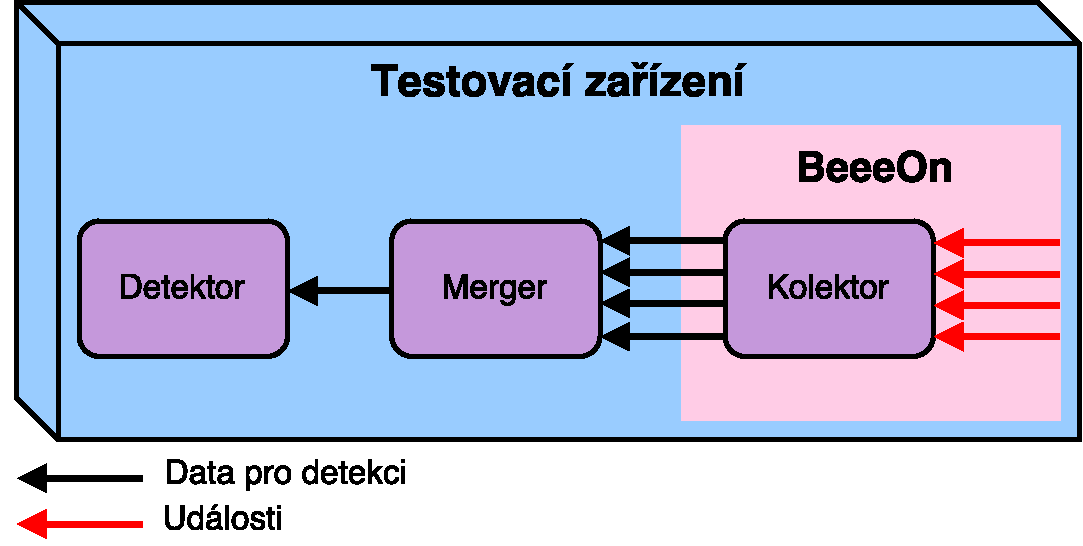
\includegraphics[scale=0.5]{pictures/deploy-option1}
   \caption{Lokální nasazení}
   \label{obr.option1}
   \end{center}
   \end{figure}
   
   Kolektor vždy odesílá dostupné události výstupními komunikačními rozhraními
   dle konfigurace brány.
   Exportovaná data přijímá NEMEA modul \textit{Merger}, který je spojuje a předává detektoru.
   
  \item \textbf{Oddělený režim} \label{externalMode}
  
  Druhý způsob nasazení byl také otestován na testovacím počítači, protože lze využít lokálních
  soketů dostupných přes NEMEA framework. Provedení realizace je na Obrázku \ref{obr.option2}.
 
  \begin{figure}[ht]
   \begin{center}
   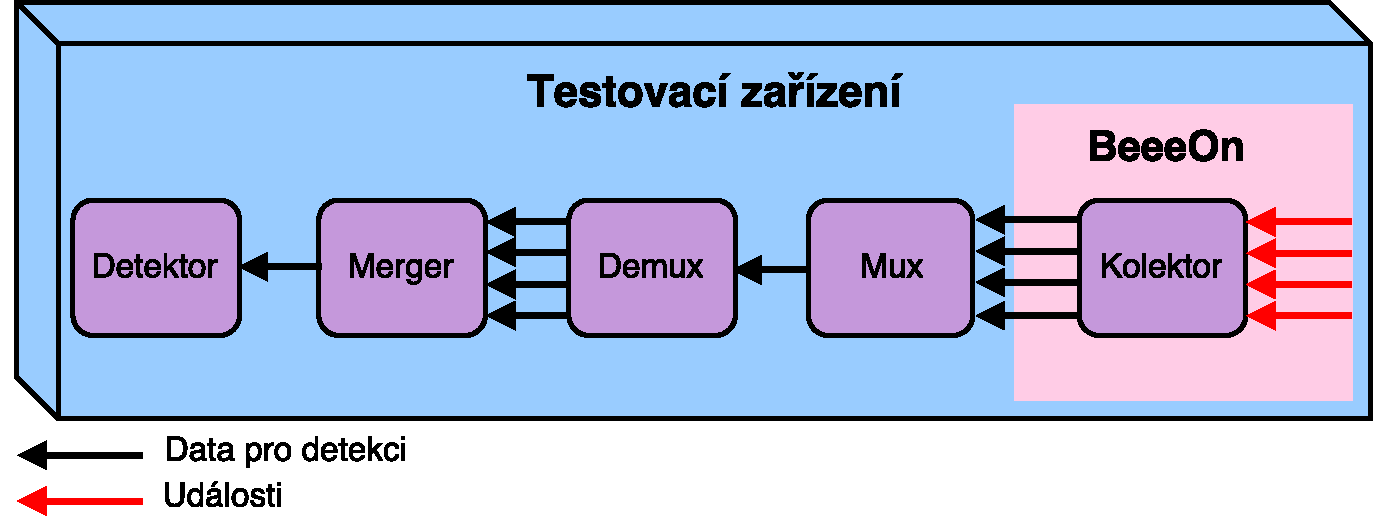
\includegraphics[scale=0.5]{pictures/deploy-option2}
   \caption{Oddělené nasazení}
   \label{obr.option2}
   \end{center}
   \end{figure}
   
   Složení komponent vychází z~prvního případu, který byl rozšířen o~moduly \textit{Mux} a 
   \textit{Demux}, které 
   umí spojit a rozdělit přicházející komunikaci.
 \end{itemize}
 
Cílem testů bylo, aby detektor obdržel všechny odeslané zprávy z~kolektoru. Ověření bylo provedeno
spuštěním detektoru s~přepínačem \textit{-vv}, který zapne ladící výpisy druhé úrovně pro zobrazení 
přijatých UniRec polí. Výsledky obou případů byly úspěšné a všechna data byla přijata.

\section{Ověření scénářů útoků} \label{testAttack}
Velmi důležitou částí bylo otestování definovaných anomálií, které mohou reprezentovat skutečný
útok na sít. Tato sekce popisuje testy pro jednotlivé scénáře.

  \begin{enumerate} [label=\textbf{S.\arabic*}]
    \item \textbf{Periodicita dat}
    
    Tento scénář nebylo nutné dělit na jednotlivé protokoly, protože popisuje obecné chování 
    připojených senzorů bez ohledu na technologii. Cílem bylo odhalit provoz, který porušuje
    očekávaný periodický průběh. V~rámci detekce nebyly potřebné naučené profily sítě, 
    ale využívalo se parametrů ze skupiny \textit{general} umožňujících periodické kontroly.
    
    První test byl určený na odhalení nepravidelného přijetí dat. Pro ověření byla použita událost
    \textit{onExport}, která poskytuje hodnoty získané ze senzorů, a v~konfiguračním souboru byla 
    aktivována pravidelná kontrola dat každých 8 sekund.
    
    Výsledek testu byl úspěšný. Pokud nebyla dodržena pravidelnost o~více než povolenou odchylku,  
    tak byly odeslány informace o~incidentu.
    
    Několik událostí poskytovaných branou BeeeOn je periodických a~po uplynutí definovaného
    času vždy odešlou dostupné statistiky. Druhý test byl zaměřen na odhalení případu, kdy se 
    přijímané datové položky nemění, což může reprezentovat odpojení nebo ztrátu čidla. Pro 
    otestování byla zvolena událost \textit{onHciStats}, která získává informace o~provozu BLE sítě. 
    Dále byla v~konfiguračním souboru nastavena pravidelná kontrola dat na 7 sekund a maximálně 
    5 po sobě přijatých hodnot mohlo být stejných. 
    
    Výsledek byl pozitivní, protože při přijetí více než pěti stejných po sobě jdoucích
    hodnot byla detekována anomálie.
    
    \item \textbf{Množství přenášených zpráv}
    
    V~případě protokolu Z-Wave byly pro nasimulování anomálií použity dvě vzdáleně ovladatelné
    zásuvky. Obě mají k~dispozici ovládací tlačítko pro vypnutí a zapnutí zásuvky. Tímto způsobem
    byly generovány nové zprávy. Cílem tohoto scénáře bylo odhalit neočekávaný nárůst dat, a~proto
    byla zvolena detekční metoda, která hlídá tyto změny. V~rámci testu byly do profilu 
    vloženy všechny dostupné položky. Limitem pro ohlášení incidentu byl pětinásobný nárůst
    provozu. Délka časové řady byla nastavena na deset prvků a prvních jedenáct přijatých 
    zpráv bylo ignorováno, protože během nich bylo navazováno spojení.
    
    První detekce byla zaměřena na položku \textit{SOAFCount}, která určuje celkový počet 
    detekovaných zpráv.  
    Druhý scénář sledoval hodnotu \textit{receivedCount}, která reprezentuje počet přijatých zpráv od
    konkrétního čidla. 
    
    Pro BLE byla časová řada zkrácena na pět prvků, žádné zprávy nebyly ignorovány a limitem
    pro určení anomálie byl dvojnásobný nárůst dat.
    Test byl proveden pro položku \textit{rxBytes}, která určuje množství obdržených zpráv.
    Údaje byly vyčítány skriptem, který v~čase měnil četnost zaslaných požadavků o~data.
    
    Výsledky testů byly úspěšné a každá změna provozu byla odhalena. Průběh všech testovaných
    případů byl velmi podobný a lišil se jen typ události a způsob generování dat. Chování 
    jednotlivých položek profilu velmi ovlivňovala délka časové řady, která určovala 
    paměťové okno. Nejcitlivější položkou na změnu byl rozptyl, který výrazně zvyšoval
    svou hodnotu při vložení vyššího čísla. K~častým výchylkám docházelo i v~případě klouzavého průměru. 
    Méně frekventované změny nastávaly u~mediánu, který nejvíce využíval délky časové řady. 
    Nejmenších odlišností dosahoval celkový průměr, protože ve své hodnotě obsahuje i data
    mimo aktuální časové okno.

    \item \textbf{Limity senzorových hodnot}
    
    Pro tento scénář byla použita data vygenerována virtuálními senzory, které jsou dostupné
    v~rámci brány BeeeOn. Do konfiguračního profilu byly vloženy všechny položky, pro které
    byly specifikovány parametry pro očekávané \textit{soft} a \textit{hard} limity. Cílem scénáře bylo odhalení
    změn v~aktuálním profilu provozu, které porušují předepsané limity. 
    
    Výsledek detekce splnil očekávání a nepovolené změny byly úspěšně detekovány. Chování 
    jednotlivých položek profilu se shodovalo s~předchozím scénářem.
    
    \item \textbf{Kvalita přenosového kanálu}
    
    Cílem tohoto scénáře bylo detekování změny kvality přenosového kanálu. Pro Z-Wave jsou 
    k~tomuto účelu vhodné položky \textit{lastResponseRTT} a \textit{dropped}. Údaj
    \textit{lastResponseRTT} je součástí události \textit{onNodeStats} a 
    \textit{dropped} je obsažen v~\textit{onDriverStats}. Z~tohoto důvodu byl při generování dat použit
    NEMEA modul \textit{Merger}, který spojil dvě různě události do jedné. Zároveň bylo nutné
    v~konfiguračním souboru
     popsat obě hodnoty. V~případě \textit{lastResponseRTT} byla jako anomálie označena
    hodnota klouzavého průměru časové řady přesahující dvojnásobek vzorového profilu a nebo byla nižší
    než polovina stanoveného klouzavého průměru. Pro položku \textit{dropped} bylo jako incident považováno
    libovolné zvětšení klouzavého mediánu. Tuto kontrolu lze nejlépe provést nastavením časového okna
    na délku jedna, položky \textit{hard} limitu na hodnotu jedna a způsobu ukládání
    na možnost \textit{delta}.
    
    Proto byla velikost časového okna rovna jedné a hard limitu byl
    nastaven na jedna. 
    
    Jelikož došlo ke spojení dvou různých událostí, kde \textit{onNodeStats}
    umožňuje získat informace pro jednotlivé senzory a \textit{onDriverStats} pro celou síť, 
    tak výsledkem byla událost poskytující informace pro každý koncový prvek. Z~tohoto důvodu 
    musel být v~konfiguraci uveden v~rámci klíče identifikátor příslušných zařízení určených k~analýze.
    
    Výstupy detekce se shodovaly s~předpoklady, a proto byl výsledek testu úspěšný. V~současné
    době se zatím nepodařilo připravit zkušební prostředí, ve které by bylo možné otestovat
    rušení kanálu, a tím ovlivnit hodnotu \textit{lastResponseRTT}. Pro účely otestování 
    detekce však byla postačující ruční úprava dat v~souboru se zachyceným provozem. 
    
    V~případě BLE by se využily položky \textit{rxErrors} nebo \textit{txErrors} a nastavení 
    detekce by bylo shodné s~\textit{lastResponseRTT}. Vzhledem k~tomu, že by došlo jen 
    ke změně názvu klíče v~konfiguračním souboru, tento test nebyl proveden.
    
    \item \textbf{Konektivita}
    
    Pro ověření posledního scénáře lze využít poznatků z~předchozích testů. Ztráta konektivity
    může být způsobena neobdržením očekávané události a to lze detekovat pomocí periodicity dat.
    Druhým způsobem je výrazné zhoršení statistik přenosového kanálu, které byly zpracovány
    v~předchozím případu užití.
  \end{enumerate}
  
  Ověření definovaných scénářů umožnilo otestování správné funkcionality vytvořeného detekčního
  systému a zároveň byla sestavena množina informací, kterou je nutné sledovat k~získání 
  přehledu o~stavu sítě.
  
  Vygenerovaný provoz, na kterém byly jednotlivé případy užití otestovány je uložen i s~nalezenými
  anomáliemi a konfiguračním souborem na přiloženém CD. V~případě testu periodicity dat nebylo možné záznam 
  komunikace uložit, protože použitá detekce využívá aktuální čas. Z~tohoto důvodu 
  byl do souboru místo záznamu uložen popis, jak takový provoz vygenerovat.

\section{Test exportu dat}
Identifikované scénáře útoků otestovaly většinu funkcí detekčního systému. Vytvořený nástroj
ovšem poskytuje i možnost pravidelného exportu definovaných položek aktuálního profilu, a tím 
vytváří informace pro další pokročilejší detekce. 

Sada testů ověřila, že vypočítané části profilu lze spolehlivě exportovat. Výsledek byl tedy
pozitivní.

\section{Měření položek profilu}
Již v~Sekci \ref{testAttack} bylo možné při ověřování scénářů sledovat odlišné chování 
jednotlivých částí profilu. V~rámci této sekce je provedeno vyhodnocení každé z~nich. Veškeré 
měření probíhalo nad stejným provozem, kde byly zprávy generovány každé tři sekundy a~pravidelné
události chodily každých pět sekund. Útoky byly reprezentovány nárůstem sledovaného provozu.
První útok byl proveden 3 minuty po zahájení komunikace a trval 90 vteřin. Druhý útok nastal 210
vteřin po prvním a trval 30 vteřin. Tyto hodnoty byly zvoleny tak, aby se projevilo co nejvíce
vlastností jednotlivých částí profilu. 

Tabulka \ref{tab.tab1} zobrazuje pro každou položku profilu míru pokrytí očekávaných detekcí obou
vygenerovaných útoků v~závislosti na 
rostoucí velikosti časové řady. Naopak Tabulka \ref{tab.tab2} obsahuje množství falešných
poplachů pro každou detekci. 

Délka časové řady nejvíce ovlivnila klouzavý medián, protože
s~rostoucí délkou se zpožďovalo rozpoznání útoku. Navíc při řadě delší než 14 prvků už nebyl rozpoznán
druhý útok, protože byl příliš krátký. Toto chování potvrzuje graf jeho průběhu
na Obrázku \ref{obr.progressMedian}, v~rámci kterého se mění měřené hodnoty skokově.

S~větší časovou řadou bylo možné uchovat i více položek, a 
tím se zvyšoval počet falešných poplachů klouzavého průměru a rozptylu, protože
v~paměťovém okně přijaté hodnoty vydržely déle. Klouzavý rozptyl byl velmi citlivý
na přijetí vyššího čísla, a proto jako jediný rozpoznal provedené útoky již od začátku. Nevýhodou
ovšem je, že při stabilním nárůstu sledované položky může jeho hodnota po uplynutí časového okna
opět klesnout do bezpečného pásma. Graf jeho průběhu na Obrázku \ref{obr.progressStandardDeviation}
zobrazuje pro větší přehlednost klouzavou směrodatnou odchylku. Klouzavý průměr během testu 
také dosahoval dobrých výsledků. Jen jeho citlivost nebyla tak výrazná, a proto při delší časové
řadě měl pomalejší reakci. Na rozdíl od klouzavého rozptylu je schopný detekovat i delší stabilní
útoky, což lze vidět na Obrázku \ref{obr.progressAverage}.

Průměr jako jediný nebyl závislý na časovém okně. Na základě tohoto předpokladu jsou v~jeho grafu
na Obrázku \ref{obr.progressCumAverage} vidět velmi pomalé a plynulé změny, které byly 
téměř konstantní při 
všech testovaných délkách. Jediným rozdílem byla delší doba učení, která stanovila vždy mírně
odlišnou hodnotu vzorového profilu.

\begin{table}[ht]
  \begin{center}
   \caption[Závislost korektně detekovaných anomálií na délce časového okna]{Tabulka obsahuje množství obdržených zpráv informujících o~detekované anomálii pro každou část profilu v~závislosti na rostoucí délce časového okna}
  \begin{tabular}{|C{1.7cm}|C{1.7cm}|C{1.7cm}|C{1.7cm}|C{1.7cm}|}
    \hline 
   \thead{velikost\\ časového\\ okna} & \thead{klouzavý\\ medián \\ {[\%]}} & \thead{klouzavý\\ rozptyl\\ {[\%]}} & \thead{klouzavý\\ průměr\\ {[\%]}} & \thead{průměr\\ {[\%]}}\\
   \hline 
   \hline 
    1 & 100 & 0 & 100 & 100\\
    \hline
    3 & 92.31 & 100 & 100 & 96.15\\
    \hline
    5 & 84.62 & 100 & 100 & 92.31\\
    \hline
    10 &  69.23 & 100 & 96.15 & 92.31\\
    \hline
    15 & 46.15 & 100 & 92.31 & 92.31\\
    \hline
    20 & 38.46 & 100 & 88.46 & 92.31\\
    \hline
   \end{tabular}
   \label{tab.tab1}
  \end{center}   
    \end{table}
    
    
    \begin{table}[ht]
  \begin{center}
   \caption[Závislost přijatých falešných poplachů na délce časového okna]{Tabulka obsahuje množství přijatých falešných poplachů pro každou část profilu v~závislosti na rostoucí délce časového okna}
  \begin{tabular}{|C{1.7cm}|C{1.7cm}|C{1.7cm}|C{1.7cm}|C{1.7cm}|}
    \hline 
   \thead{velikost\\ časového\\ okna} & \thead{klouzavý\\ medián \\ {[\%]}} & \thead{klouzavý\\ rozptyl\\ {[\%]}} & \thead{klouzavý\\ průměr\\ {[\%]}} & \thead{průměr\\ {[\%]}}\\
   \hline 
   \hline 
    1 & 0 & 100 & 0 & 0\\
    \hline
    3 & 7.69 & 13.33 & 13.33 & 72.22\\
    \hline
    5 & 15.38 & 23.53 & 20 & 73.03\\
    \hline
    10 &  30.77 & 40.91 & 37.50 & 73.03\\
    \hline
    15 & 36.84 & 48.15 & 50 & 73.03\\
    \hline
    20 & 47.37 & 58.06 & 58.93 & 73.03\\
    \hline
   \end{tabular}
   \label{tab.tab2}
  \end{center}   
    \end{table}


    \begin{figure}[ht]
   \begin{center}
   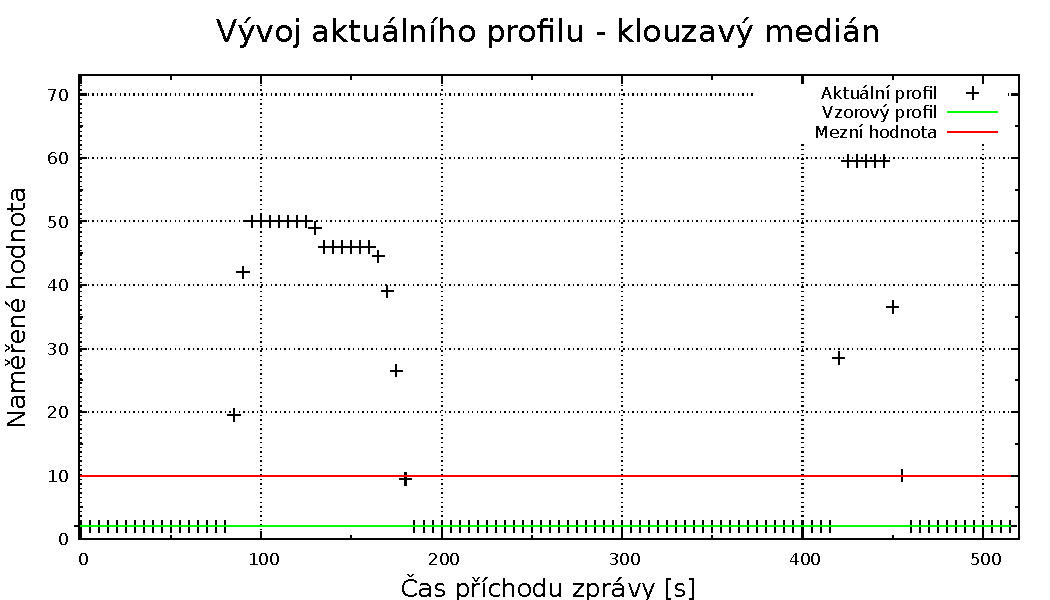
\includegraphics[scale=0.7]{pictures/moving_median_progress}
   \caption[Graf vývoje klouzavého mediánu]{Graf vývoje klouzavého mediánu s~časovou řadou délky 10}
   \label{obr.progressMedian}
   \end{center}
   \end{figure}
   
   \begin{figure}[ht]
   \begin{center}
   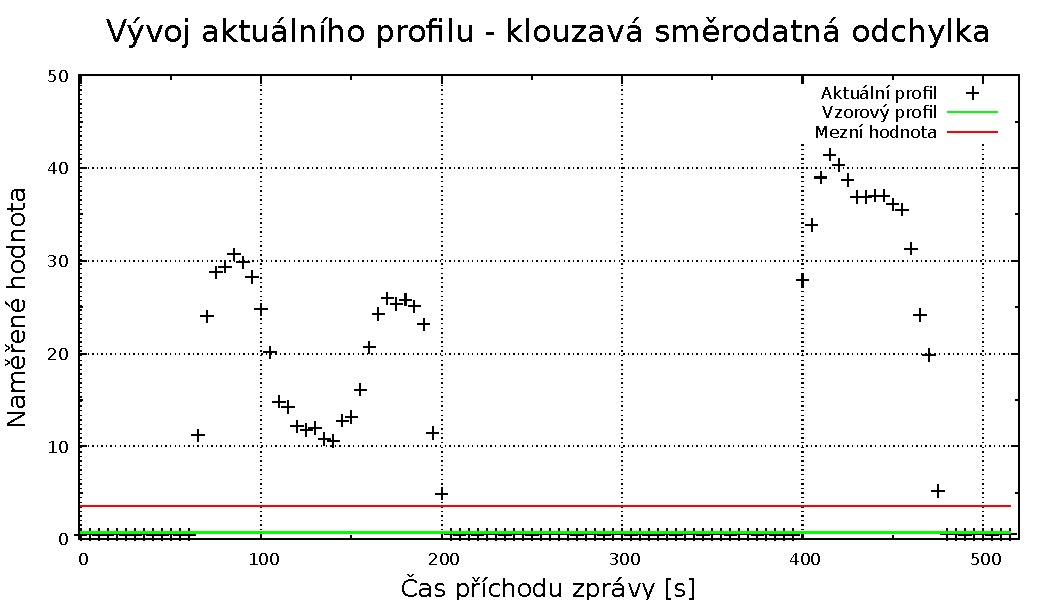
\includegraphics[scale=0.7]{pictures/moving_standard_deviation_progress}
   \caption[Graf vývoje klouzavé směrodatné odchylky]{Graf vývoje klouzavé směrodatné odchylky s~časovou řadou o~délce 10}
   \label{obr.progressStandardDeviation}
   \end{center}
   \end{figure}
    
  \begin{figure}[ht]
   \begin{center}
   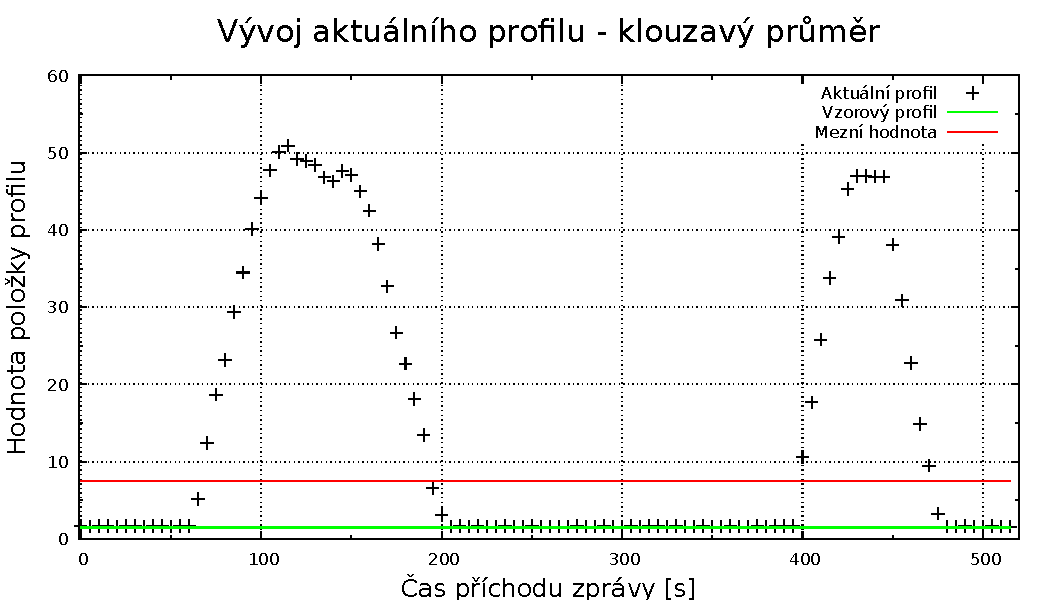
\includegraphics[scale=0.7]{pictures/moving_average_progress}
   \caption[Graf vývoje klouzavého průměru]{Graf vývoje klouzavého průměru s~časovou řadou délky 10}
   \label{obr.progressAverage}
   \end{center}
   \end{figure}
   
   \begin{figure}[ht]
   \begin{center}
   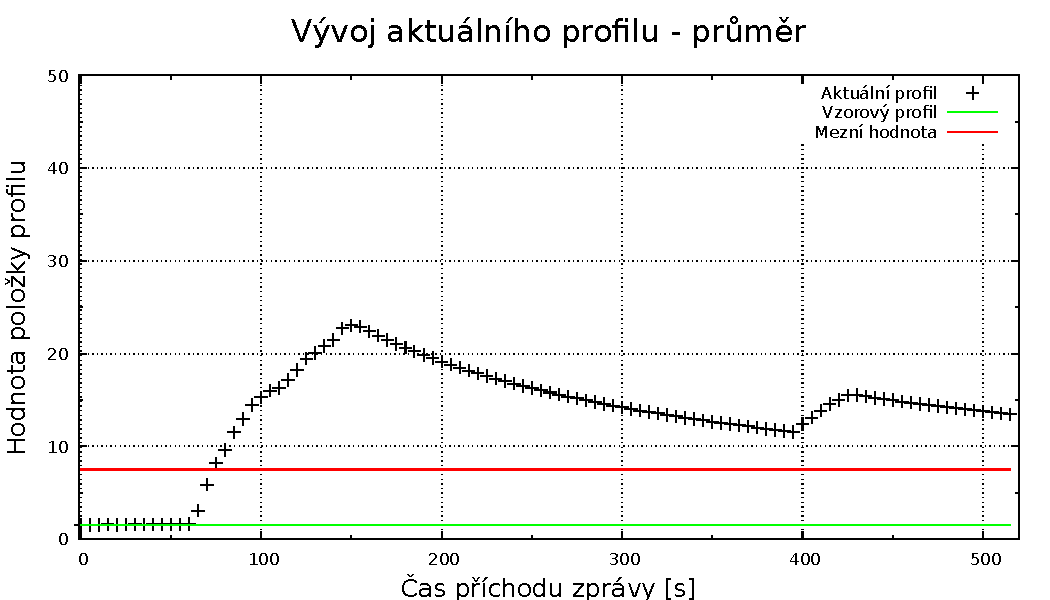
\includegraphics[scale=0.7]{pictures/average_progress}
   \caption[Graf vývoje průměru]{Graf vývoje průměru s~časovou řadou délky 10}
   \label{obr.progressCumAverage}
   \end{center}
   \end{figure}

\begin{conclusion}

Cílem diplomové práce bylo analyzovat aktuální stav IoT sítí a identifikovat bezpečnostní 
slabiny. Na základě získaných znalostí byl navržen,
implementován a otestován nástroj
pro monitorování a automatickou detekci anomálního provozu. Výsledný nástroj se skládá z~několika
komponent, které komunikují pomocí systému NEMEA a rozšiřují funkcionalitu IoT brány BeeeOn
o~možnost detekce. 

V~první části této práce byl představen koncept fog computingu, který mění 
způsob zpracování dat v~IoT sítích. Dále byly popsány jednotlivé komunikační vrstvy a detailně rozebrány
aktuálně používané protokoly včetně jejich bezpečnostních slabin. Následně byla věnována 
pozornost možným způsobům detekce útoků a také byly hledány již existující nástroje 
pro řešení této 
problematiky, které v~současnosti nedostatečné pokrývají možné hrozby. Nejméně pokrytá byla 
senzorová vrstva, kde jsou nejzranitelnější bezdrátové komunikační protokoly, které jsou zároveň 
pro svou mobilitu velmi často používané.
V~závěru jsou uvedeny
požadavky na výsledný program a vhodné technologie pro vývoj.

Při návrhu byly splněny všechny kladené nároky a výsledné řešení bylo navrženo tak, aby jej 
bylo možné nasadit i na IoT branách s~omezenými prostředky nebo v~decentralizovaném prostředí. 
Dále byly popsány scénáře útoků, které se mohou objevit při reálném provozu v~senzorové vrstvě.
V~rámci scénářů byla sestavena množina informací, které je potřeba měřit k~získání přehledu
o~stavu sítě. 

Vzhledem k~pečlivě provedenému návrhu nebylo nutné během implementace řešit žádné problémy. Naopak
díky použitému frameworku NEMEA bylo spoustu věcí usnadněno. Při 
realizaci byly splněny všechny funkční i nefunkční požadavky, které dokonce přesahují nároky 
specifikované v~zadaní práce.

Velký důraz byl kladen na testování, které odhalilo řadu implementačních chyb, ale všechny byly
opraveny. V~rámci testů bylo ověřeno úspěšné detekování navržených scénářů útoků, byly
otestovány způsoby nasazení a~také bylo provedeno měření chování položek profilu sítě.

Zpracování této diplomové práce mělo pro mě velký přínos. Dozvěděl jsem se mnoho nových znalostí 
z~oblasti IoT, které jsem si navíc prakticky vyzkoušel. Tato oblast se bude v~dalších
letech rozšiřovat, a proto se získané zkušenosti budou velmi hodit v~dalších projektech.

\section{Budoucí práce}
V~následujících letech je očekáváno velké rozšíření IoT sítí, které jsou řízeny člověkem a 
konfigurovány strojem. Z~tohoto důvodu má tato práce velký potenciál, protože tuto oblast pokrývá
teoretickým i praktickým směrem a může být využita jako základ pro budoucí práce. 

Jedním ze způsobů
rozšíření je použití dalších detekčních metod, které budou využívat externí sondy pro získávání
podrobnějších informací o~daném protokolu. Tyto sondy zároveň mohou sloužit jako honeypoty.

Dalším rozšířením může být externí nástroj, který se bude starat o~generování konfigurace pro 
vytvořený detektor. Generátor nastavení bude velmi vhodný pro koncové uživatele, protože si budou
moci přehledně vybrat své parametry bez znalosti všech závislostí, které textová varianta ani 
modul pro zpracování nehlídá. 

Vytvořený program zároveň umožňuje pravidelně 
získávat informace o~profilu sítě, které mohou být využity k~sestavení datového modelu. 
Následně při použití
analytických metod lze provádět pokročilé způsoby detekce.

Důležité bude také pokrytích další komunikačních protokolů, které zahrnují i protokoly síťové 
vrstvy. Pro síťové protokoly může být vhodné využít principů nástroje \textit{Joy} \cite{joy}, 
který se zaměřuje 
na vyhodnocování incidentů v~šifrovaném provozu.
\end{conclusion}

\bibliographystyle{csn690}
\bibliography{mybibliographyfile}

\appendix

\chapter{Seznam použitých zkratek}
% \printglossaries
\begin{description}
	\item[IoT] Internet of Things
	\item[IP] Internet Protocol
	\item[HTTPS] Hypertext Transfer Protocol Secure  
	\item[VPN] Virtual Private Network 
	\item[MQTT] Message Queuing Telemetry Transport 
	\item[CoAP] Constrained Application Protocol 
	\item[AMQP] Advanced Message Queuing Protocol
	\item[DDoS] Distributed Denial Of Service
	\item[MITM] Man In The Middle
	\item[M2M] Machine To Machine 
	\item[TCP] Transmission Control Protocol
	\item[QoS] Quality of Service
	\item[TLS] Transport Layer Security
	\item[RESTful] Representational State Transfer
	\item[UDP] User Datagram Protocol
	\item[HTTP] Hypertext Transfer Protocol
	\item[URI] Uniform resource identifier
	\item[DTLS] Datagram Transport Layer Security
	\item[ISM] Industrial, Scientific and Medical
	\item[AES] Advanced Encryption Standard
	\item[PIN] Personal Identification Number
	\item[QR] Quick Response
	\item[ECDH] Elliptic-curve Diffie–Hellman
	\item[BLE] Bluetooth Low Energy 
	\item[SIG] Special Interest Group
	\item[NFC] Near Field Communication
	\item[IDS] Intrusion Detection System
	\item[IPS] Intrustion Prevention System
	\item[SCADA] Supervisory Control And Data Acquisition
	\item[NEMEA] Network Measurements Analysis
	\item[UniRec] Unified Record
	\item[RAII] Resource Acquisition Is Initialization
	\item[RTT] Round-Trip Time
\end{description}

\chapter{Instalační příručka}
Realizovaný detekční systém pro svůj běh využívá framework NEMEA a projekt BeeeOn. V~následujících
krocích je popsána instalace těchto dvou nástrojů, způsob nasazení kolektoru a
spuštění detekčních modulů.

\begin{enumerate}
 \item \textbf{Instalace projektu BeeeOn}
 
 Zdrojové kódy tohoto projektu se nachází v~repozitáři služby Github. Pro jeho sestavení je nutné
 vykonat následující příkazy: 
\begin{verbatim}
git clone https://github.com/BeeeOn/gateway.git --recursive
cd  gateway
mkdir build
(cd build && cmake ..)
make -C build
\end{verbatim}
 \item \textbf{Instalace NEMEA frameworku}
 
Kompletní zdrojové kódy systému NEMEA jsou také udržovány v~repozitářích služby Github. Pro
vytvořený nástroj je potřeba nasadit část \textit{NEMEA-Framework}.
\begin{verbatim}
git clone https://github.com/CESNET/Nemea-Framework.git
cd Nemea-Framework
./bootstrap.sh
./configure
make
sudo make install
\end{verbatim}

Pro spouštění vytvořených testů nebo pro úpravu příchozích a odchozích dat ve formátu UniRec se
mohou hodit moduly \textit{Logger}, \textit{Logreplay} a~\textit{Merger}, které se nacházejí
v~částí \textit{NEMEA-Modules}. V~tomto 
repozitáři se zároveň nachází vytvořené moduly \textit{Mux} a \textit{Demux}.
\begin{verbatim}
git clone https://github.com/CESNET/Nemea-Modules.git
cd Nemea-Modules
./bootstrap.sh
./configure
make
sudo make install
\end{verbatim}

\item \textbf{Nasazení kolektoru}

V~rámci tohoto kroku je potřeba zdrojové kódy vytvořeného kolektoru přesunout do BeeeOn brány
a upravit konfigurační soubory. Postup je popsán v~následujících sekcích.
\begin{itemize}
 \item \textbf{Přesun zdrojových souborů}
\begin{verbatim}
   cp NemeaCollector.* <adresářBeeeOn>/src/core
   cp fields.* <adresářBeeeOn>/src/core
\end{verbatim}
\item \textbf{Úprava souborů pro kompilaci}
\begin{verbatim}
   vim <adresářBeeeOn>/src/CMakeLists.txt
\end{verbatim}
Do příslušných částí v~souboru je potřeba vložit tyto položky: 
\begin{verbatim}
   find_library (LIBTRAP trap)
   find_library (UNIREC unirec)
   find_library (PCAP pcap)

   ${PROJECT_SOURCE_DIR}/core/fields.cpp
   ${PROJECT_SOURCE_DIR}/core/NemeaCollector.cpp

   ${PCAP}
   ${UNIREC}
   ${LIBTRAP}
\end{verbatim}
Podobné změny je nutné provést v adresáři \textit{test}
\begin{verbatim}
  vim <adresářBeeeOn>/test/CMakeLists.txt
    find_library (LIBTRAP trap)
    find_library (UNIREC unirec)
    find_library (PCAP pcap)
    
    ${PCAP}
    ${UNIREC}
    ${LIBTRAP} 
\end{verbatim}
 \item \textbf{Úprava sestavovací konfigurace brány}
\begin{verbatim}
   vim <adresářBeeeOn>/conf/config.d/factory.xml 
\end{verbatim}
V otevřeném souboru je nutné do odpovídajících elementů vložit tyto parametry:
\begin{verbatim}
   #element instance name="distributor"
   <add name="listener" ref="collector"/>

   #element instance name="bluetoothAvailability"
   <add name="listeners" ref="collector"/>

   #element instance name="zwaveDeviceManager"
   <add name="listeners" ref="collector"/>

   #element instance name="commandDispatcher"
   <add name="listeners" ref="collector"/>

   #element factory
   <instance name="collector" 
             class="BeeeOn::NemeaCollector">
     <set name="onExportInterface" 
          text="u:event-onExport"/>
     <set name="onHCIStatsInterface" 
          text="u:event-onHCIStats"/>
     <set name="onDispatchInterface" 
          text="u:event-onDispatch"/>
     <set name="onNodeStatsInterface" 
          text="u:event-onNodeStats"/>
     <set name="onDriverStatsInterface" 
          text="u:event-onDriverStats"/>
   </instance> 
\end{verbatim} 
\item \textbf{Rekompilace brány}
\begin{verbatim}
   cd <beeeonRootDir>
   (cd build && cmake ..)
   make -C build
\end{verbatim}
\end{itemize}

\item \textbf{Kompilace detektoru}

Kompilace komponenty detektoru se provede následujícím příkazem:
\begin{verbatim}
g++ DataDetector.cpp fields.cpp ConfigParser.cpp \
Analyzer.cpp -o prg -ltrap -lpcap -lunirec --std=c++11 \
-Wno-write-strings -pthread 
\end{verbatim}
\newpage
\item \textbf{Spuštění detekčního systému}

Posledním krokem je spuštění celého detekčního systému. Pro účely demonstrace je
v~ukázce použit oddělený model nasazení \ref{externalMode}, který zahrnuje více komponent. Při reálném 
použití stačí spustit pouze kolektor a jednu instanci detektoru pro každý typ události. V~uvedené
ukázce každá z~komponent používá standardní výstup, proto je nutné každý příkaz spustit v~samostatném
terminálovém okně.
\begin{verbatim}
<adresářBeeeOn>/build/src/beeeon-gateway \
   -c conf/gateway-testing.ini -Dtesting.center.enable=yes 
mux "u:event-onDriverStats,u:event-onNodeStasts,u:output" \
   -n 2
demux -i "u:output,u:onDriverStats,u:onNodeStats" -n 2
merger -i "u:onDriverStats,u:onNodeStats,u:merged" -n 2
<adresářDetector>/prg -i "u:merged,u:alert" -v
logger -i "u:alert" -t
logger -i "u:export-dropped0" -t
\end{verbatim}
\end{enumerate}


\chapter{Nástroje pro testování}
V~následující kapitole přílohy se nachází popis způsobu použití nástrojů, které byly uplatněny 
v~rámci testování.

\begin{itemize}
 \item \textbf{Logger}

 Tento NEMEA modul slouží k~ukládání přijatých UniRec zpráv. Při spuštění je nutné zadat 
 přepínač \textit{-i} s~popisem vstupního komunikačního rozhraní. Dále je dobré použít přepínač
 \textit{-w <názevSouboru>} pro ukládání přijatých dat do souboru, \textit{-t} pro uložení datové
 hlavičky příchozích
 dat a \textit{-T}, který ukládá i časové značky.
 
 Příklad spuštění: \textit{logger -t -T -i u:alert -w alert-data.log}
 
 \item \textbf{Logreplay}
 
 Modul \textit{Logreplay} lze využít pro přehrání zachyceného provozu pomocí modulu \textit{Logger}.
 Mezi povinné
 přepínače patří
 \textit{-i}, za kterým následuje popis výstupního komunikačního rozhraní, a \textit{-f <názevSoboru>}
 pro načtení
 uloženého provozu. Vhodným přepínačem může být \textit{-n}, který neposílá po přehrání EOF (End Of File)
 zprávu. Pokud soubor se zachycenými daty obsahuje časové značky každého záznamu, tak jsou 
 jednotlivé zprávy odesílány dle těchto značek.
 
 Ukázka použití: \textit{logreplay -i u:zwave -f z-wave-connection.log -n}
 
 \item \textbf{Merger}
 
 Poslední uvedený NEMEA modul se používá pro slučování několika různých vstupních UniRec
 záznamů do jednoho společného, který je odesílán výstupním rozhraním. Očekávanými parametry jsou
 \textit{-i} s~popisem komunikačního rozhraní a \textit{-n} určující počet vstupních rozhraní,
 který odpovídá
 zadanému popisu. Název výstupu je vždy uveden jako poslední položka v~rámci přepínače \textit{-i}.
 
 Možné zavedení: \textit{merger u:DriverStasts,u:NodeStats,u:merged -n 2}
 

\end{itemize}


\chapter{Popis množiny senzorových informací} \label{sensorData}
Tato část přílohy obsahuje kompletní popis množiny informací, kterou lze v~současné době získat
o~provozu senzorových protokolů v~rámci BeeeOn brány. Při popisu byla množina informací rozdělena
do příslušných událostí, které
jsou reprezentovány samostatnou sekcí.

\section{onDriverStats}
\begin{description}
 \item \textbf{SOAFCount}: počet přijatých Start Of Frame bytů
 \item \textbf{ACKWaiting}: počet nevyžádaných zpráv při čekání na potvrzení
 \item \textbf{readAborts}: počet nedokončených operacích čtení z~důvodu překročení časového limitu
 \item \textbf{badChecksum}: počet zpráv se špatných kontrolním součtem
 \item \textbf{readCount}: počet úspěšně přijatých zpráv
 \item \textbf{writeCount}: počet úspěšně odeslaných zpráv
 \item \textbf{CANCount}: počet přijatých CAN bytů
 \item \textbf{NAKCount}: počet přijatých negativních potvrzení
 \item \textbf{ACKCount}: počet přijatých potvrzení
 \item \textbf{OOFCount}: počet přijatých Out Of Frame bytů
 \item \textbf{dropped}: počet zahozených zpráv 
 \item \textbf{retries}: počet znovu odeslaných zpráv
 \item \textbf{callbacks}: počet neočekávaných callbacků
 \item \textbf{badroutes} počet neodeslaných zpráv kvůli směrování
 \item \textbf{noACK}: počet neobdržených potvrzení
 \item \textbf{netBusy}: počet zpráv s~chybovým stavem
 \item \textbf{notIdle}: počet zpráv se stavem not idle
 \item \textbf{nonDelivery}:počet nedoručených zpráv
 \item \textbf{routedBusy}:  počet přijatých zpráv se stavem routed busy
 \item \textbf{broadcastReadCount}: počet přijatých všesměrových zpráv
 \item \textbf{broadcastWriteCount}:počet odeslaných všesměrových zpráv
\end{description}

\section{onNodeStats}
\begin{description}
 \item \textbf{sentCount}: počet odeslaných zpráv
 \item \textbf{sentFailed}: počet zpráv, které se nepodařilo odeslat
 \item \textbf{receivedCount}: počet přijatých zpráv
 \item \textbf{receivedDuplications}: počet přijatých duplikovaných zpráv
 \item \textbf{receivedUnsoliced}: počet přijatých nevyžádaných zpráv
 \item \textbf{lastRequestRTT}: RTT poslední odeslané zprávy
 \item \textbf{lastResponseRTT}: RTT poslední přijaté odpovědi
 \item \textbf{averageRequestRTT}: průměr z~lastRequestRTT
 \item \textbf{averageResponseRTT}: průměr z~lastResponseRTT
 \item \textbf{quality}: kvalita připojení
 \item \textbf{nodeID}: identifikátor senzoru
\end{description}

\section{onHCIStats}
\begin{description}
 \item \textbf{address}: adresa BLE rozhraní 
 \item \textbf{aclMtu}: velikost MTU pro ACL zprávy
 \item \textbf{aclPackets}: velikost zásobníku pro ACL zprávy 
 \item \textbf{scoMtu}: velikost MTU pro SCO zprávy
 \item \textbf{scoPackets}: velikost zásobníku pro SCO zprávy
 \item \textbf{rxErrors}: počet přijatých chybových zpráv
 \item \textbf{txErrors}: počet odeslaných chybových zpráv
 \item \textbf{rxEvents}: počet přijatých BLE událostí
 \item \textbf{txCmds}: počet odeslaných BLE příkazů
 \item \textbf{rxAcls}: počet přijatých ACL zpráv
 \item \textbf{txAcls}: počet odeslaných ACL zpráv
 \item \textbf{rxScos}: počet přijatých SCO zpráv
 \item \textbf{txScos}: počet odeslaných SCO zpráv
 \item \textbf{rxBytes}: počet přijatých bytů
 \item \textbf{txBytes}: počet odeslaných bytů
\end{description}

\section{onExport}
\begin{description}
 \item \textbf{value}: senzorová hodnota
 \item  \textbf{deviceID}: identifikátor senzoru
\end{description}

\chapter{Obsah přiloženého CD}

\begin{figure}
	\dirtree{%
		.1 readme.txt\DTcomment{stručný popis obsahu CD}.
		.1 src\DTcomment{zdrojové soubory}.
		.2 impl\DTcomment{zdrojové kódy implementace}.
		.3 collector\DTcomment{zdrojové kódy kolektoru}.
		.3 detector\DTcomment{zdrojové kódy detektoru}.
		.3 mux\DTcomment{zdrojové kódy multiplexoru}.
		.3 demux\DTcomment{zdrojové kódy demultiplexoru}.
		.3 test\DTcomment{soubory pro testování}.
		.2 thesis\DTcomment{zdrojová forma práce ve formátu \LaTeX{}}.
		.1 text\DTcomment{text práce}.
		.2 DP\_Soukup\_Dominik.pdf\DTcomment{text práce ve formátu PDF}.
		.2 ZadaniDP\_Soukup\_Dominik.pdf\DTcomment{zadání práce ve formátu PDF}.
	}
\end{figure}

\end{document}
